\chapter{Cryostat Configuration}
\label{Sec:cryo-cryosys-cryostat}

\section{Sides and Bottom of Cryostat}

The membrane cryostat is a sealed container that relies on external support 
from the surrounding steel frame (outer warm vessel) to resist the hydrostatic 
load of the contents. From innermost to outermost layers, the side 
walls of the membrane cryostat consist of 
\begin{itemize}
 \item{the stainless-steel primary membrane} 
 \item{insulation (inner layer)}
 \item{a secondary barrier (thin aluminum membrane that contains the 
       LAr in case of a leak in the primary membrane)}
 \item{more insulation (outer layer)}
 \item{a barrier to prevent water-vapor ingress to the cryostat}
 \item{the steel frame (outer warm vessel)}
\end{itemize}  
%The membrane cryostat is considered a ``full containment'' 
%system in the LNG industry lexicon.
The basic components of the membrane cryostat are illustrated in
Figure~\ref{fig:composite-sys-install}. The cryostat is positioned
inside the rock pit with enough air space reserved for convection
or forced air circulation, which maintains rock temperatures above
freezing.

\begin{figure}[htbp]
\centering
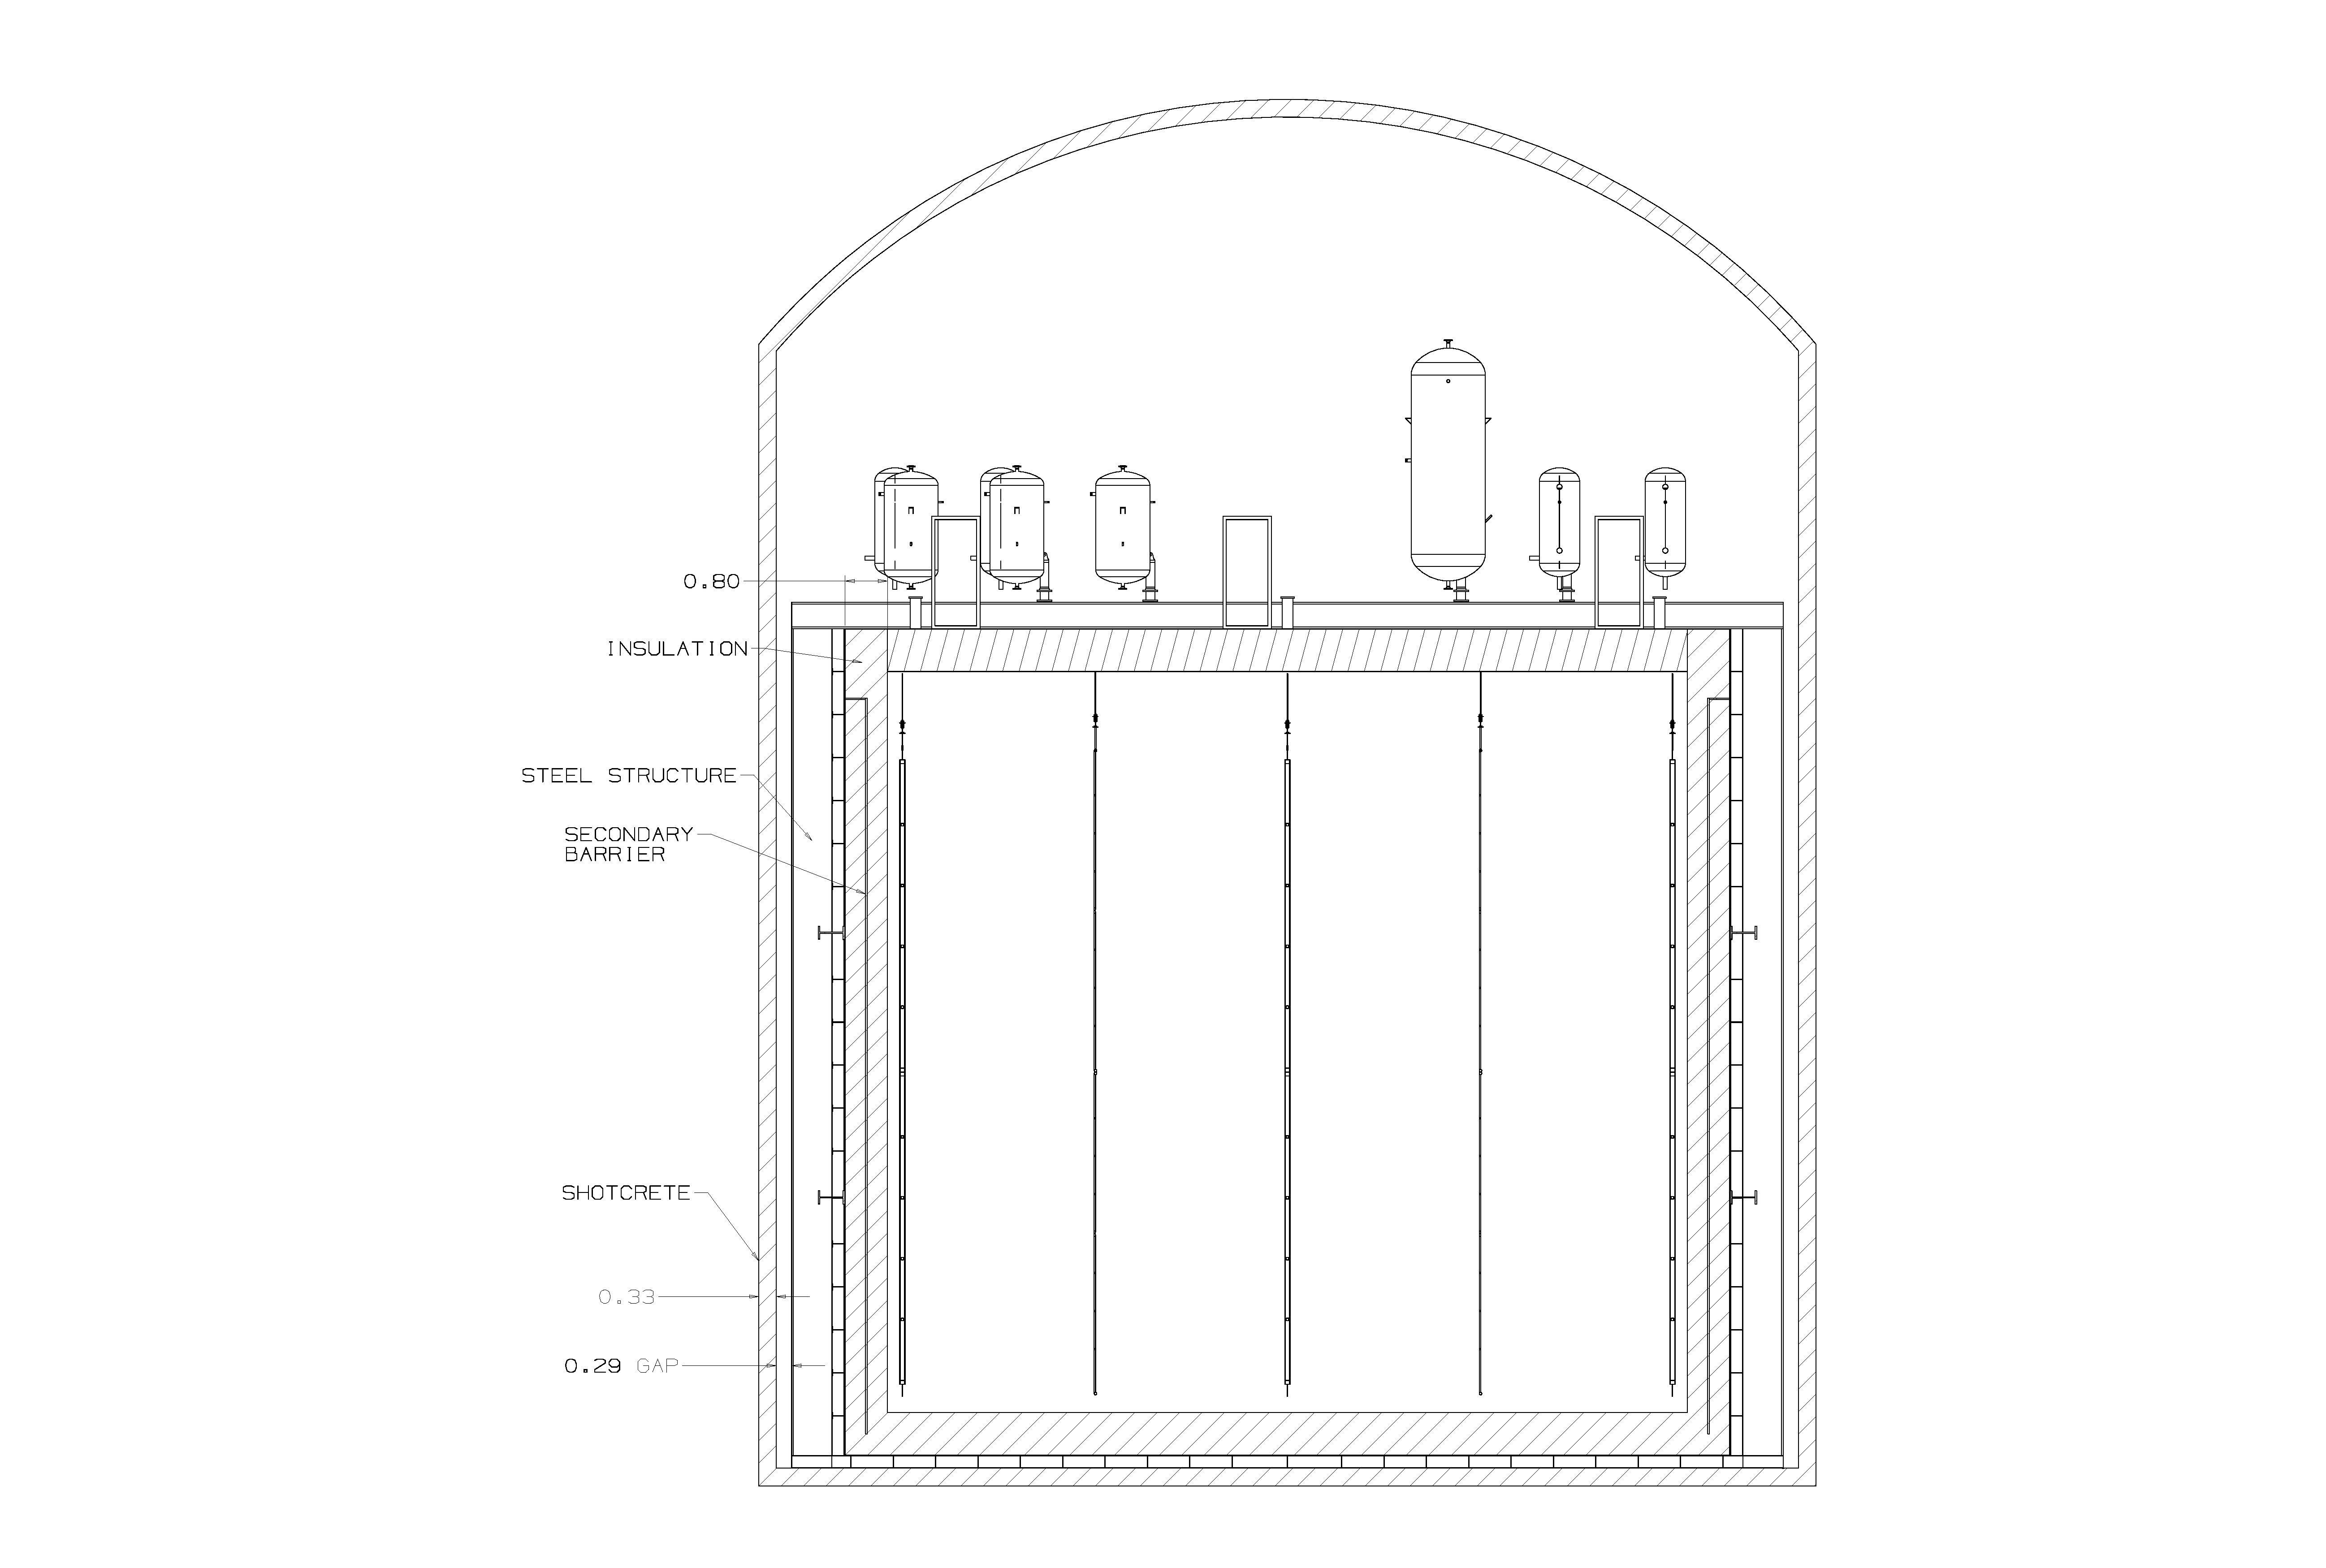
\includegraphics[width=\textwidth]{composite-sys-install}
\caption{Composite system as installed for the LBNF reference design} 
\label{fig:composite-sys-install}
\end{figure}


\section{Steel Frame and Vapor Barrier}
%The formed concrete liner will be poured against the sides 
%and bottom of the excavated rock pit. Conduits and heating 
%elements will be embedded in the concrete liner

%The embedded conduits are encased approximately midway in 
%the concrete side walls, end walls and bottom floor slab 
%as depicted in Figure~\ref{fig:endview-liner}. 
%The concrete liner and conduits are provided under the 
%conventional facilities scope. The heating elements are 
%provided by LBNF scope.
A vapor barrier is required on all internal surfaces of the 
steel frame (base, side walls, and end walls) and the roof to 
prevent the ingress of any water vapor into the insulation 
space. If water vapor were permitted to migrate into the 
insulation space, it could freeze and degrade the thermal 
performance of the insulation. The barrier must also 
reliably absorb the stresses and strains from all normal 
loading conditions. The selected vapor barrier material 
is a stainless steel plate of 10 mm applied to the side,
top and bottom surfaces. 

Each of the four identical cryostats will consist of two 
major components: a steel outer frame (warm vessel) and 
membrane cold vessel. The membrane cold vessel is based 
on the technology used for liquefied natural gas (LNG) 
storage and transport ships. It consists of an inner 
stainless steel corrugated thin membrane in contact with 
the liquid and thermal insulation surrounding it. Details 
of this technology are presented in Chapter~\ref{ch:cryo-intro}. 
The main idea behind this concept is that the cold membrane vessel 
represents a fully contained vessel with two independent 
barriers.

The function of steel warm vessel is to contain the membrane 
vessel and provide mechanical support to it, while providing 
also a gas barrier towards the outside. Figure~\ref{fig:SteelVessel} 
below presents the layout of such an assembly which consists
of a modular self-supporting steel structure.

\begin{figure}[htbp]
\centering
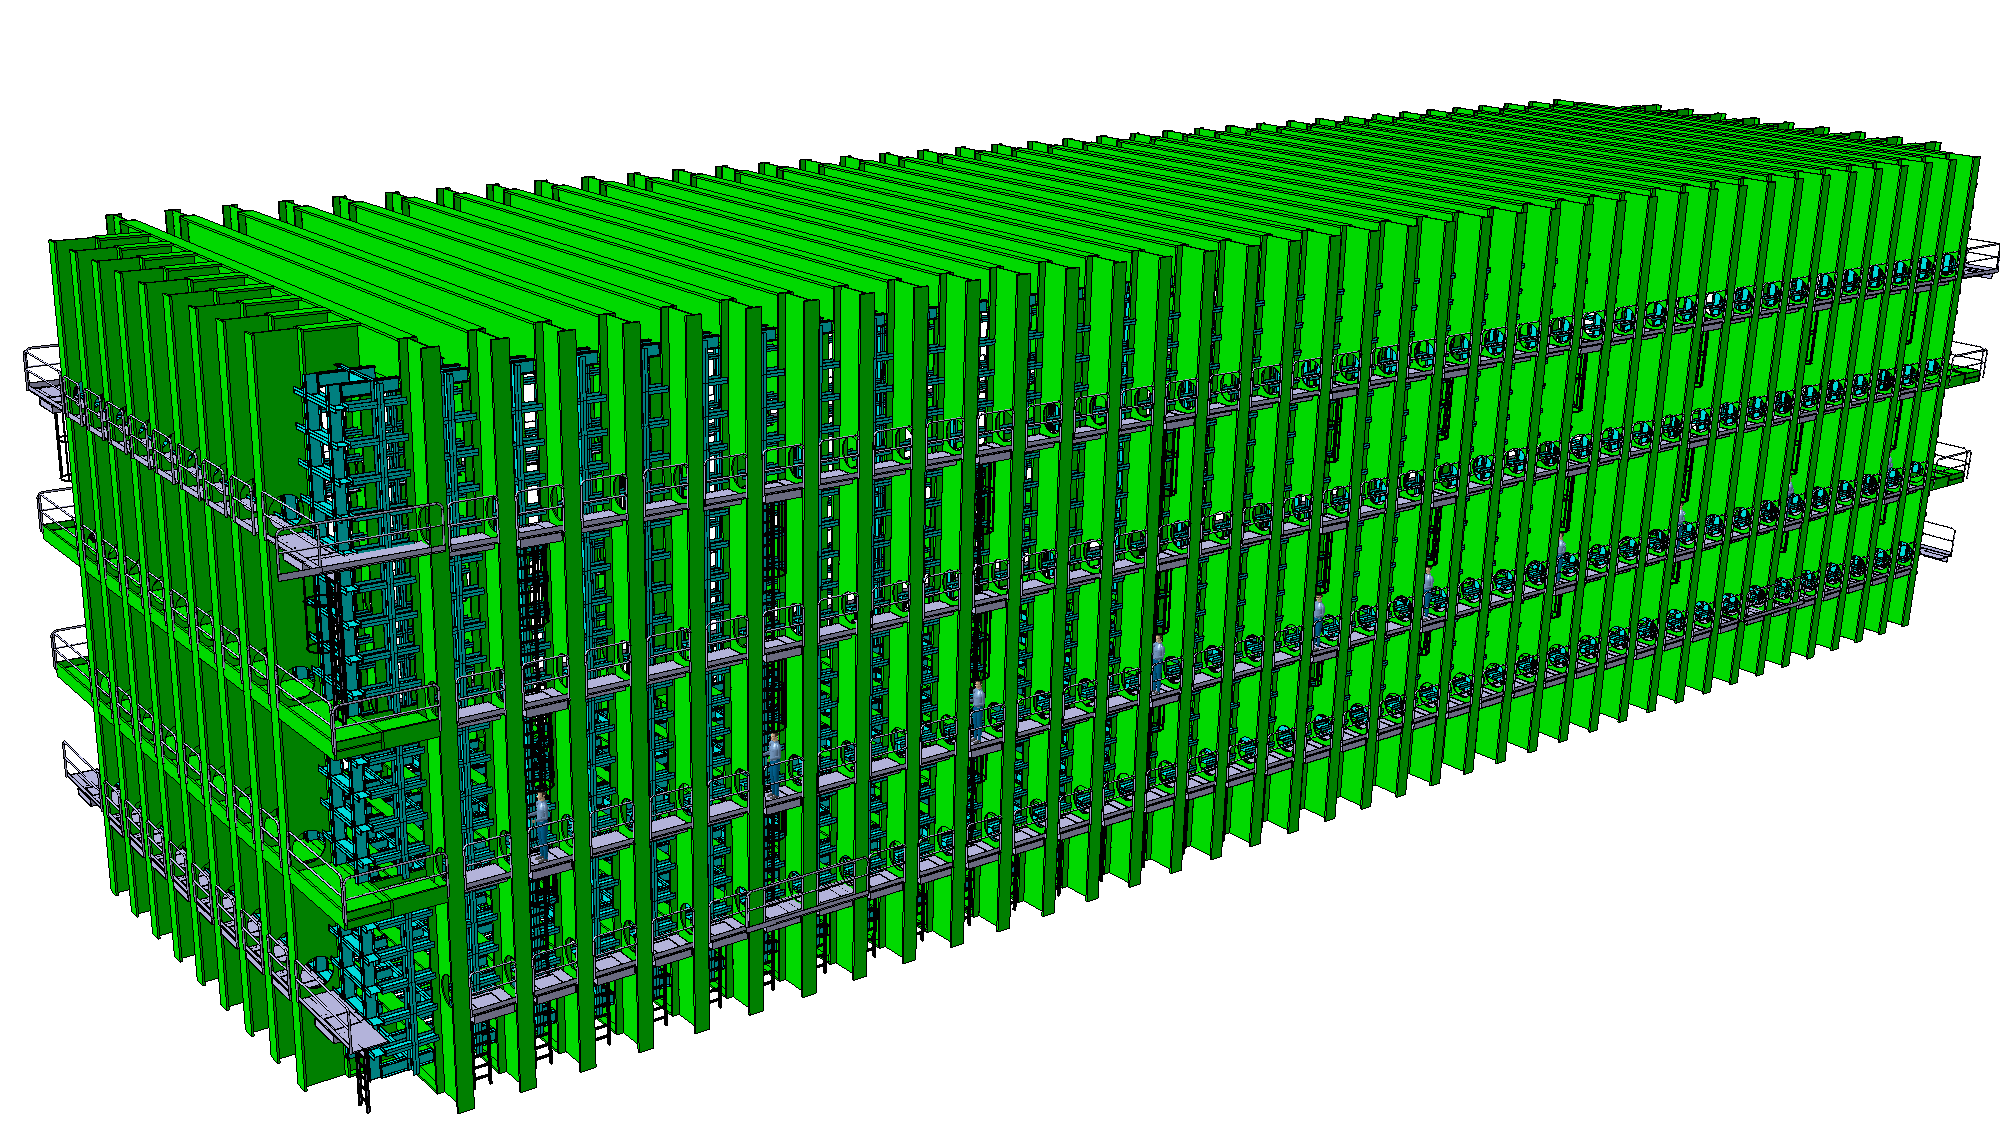
\includegraphics[width=0.85\textwidth]{SteelVessel}
\caption[Outer layout of steel warm vessel]{Outer layout of steel warm vessel}
\label{fig:SteelVessel}
\end{figure}

The structure will be positioned on a firm surface with 
no additional structural connections necessary for either 
the cavern floor or the cavern walls. The internal (external) 
dimensions of the structure are approximately 16.9 (19.0) m 
in width, 15.8 (18.0) m in height, and 63.8 (66.0) m in length.

The warm vessel consists of outer supporting profiles, interconnected 
through a steel grid and a 10 mm thick stainless steel (type 304L) 
continuous plate to the inside in contact with the membrane insulation.
The material used is S460ML structural carbon steel, with yield 
strength of 430 MPa and tensile strength of 510 MPa. The main 
profile used is HL 1100$\times$548 or its ASTM alternative 
W 44$\times$16$\times$368. Four profiles are bolted together, by 
four bolting connections, forming a structural "portal". Each 
bolting connection consists of 16 bolts (M42). The additional 
grid is made of the IPE300 profile. The total self-weight of 
the structure is approximately 2000 T.

The main advantage of this design is the fact that such a structure 
can be fully decoupled from the civil engineering work related to
the excavation and finishing of the four caverns. All components 
can be procured and prepared on the surface, ready to be lowered 
through the shaft. Underground installation will take 4 
months for each of the cryostats and can be done sequentially.  
The warm vessel will be fully accessible from outside and can be 
inspected at any moment. A net of stairs and gangways is included 
in the design at the allocated space. No requirements are put on 
the distance of the warm structure to the cavern walls. Typically
 this value might vary between 200 and 500 mm. The warm cryostat 
is positioned inside the cavern pit with enough air space 
reserved for convection or forced air circulation, which maintains 
the rock temperatures above freezing.

Finite Elements Analysis Methods using the commercial ANSYS code 
have been employed as the main design technique. The safety codes 
used are the Eurocode III and ASME Boiler and Pressure Vessel code 
Section VIII, Rules for Construction of Pressure Vessel, 
Division II. The most conservative requirements among the two 
codes have been adopted. The structure has been treated as a 
low pressure vessel (<500 mbarg). 

Approximately 18000 T of LAr is acting as load on the floor, i.e. 
around 20 T/m$^{2}$. Approximately 8000 T of hydrostatic force is acting 
on each of the long walls, with triangular distribution over the 
height, and around 2000 T of hydrostatic force is acting on each 
of the short walls.  Additionally a normal ullage operational pressure 
of 75 mbarg (0.75 T/m$^{2}$) is considered, acting in addition on every 
wall. The structure has been also verified to accidental overpressure 
of 350 mbarg (3.5 T/m$^{2}$), which is the maximum allowable working pressure 
of the cryostat.  The weight of the detector itself, as well as 
seismic action, has been taken into account in the calculations.

The following models and analyses methods have been utilized:
\begin{itemize}
 \item{For evaluation of the global behavior of the entire structure,
       a beam model has been developed.}
 \item{Analytical models of a single portal, i.e. 4 main beams 
       connected together (roof, floor and the side walls) 
       have been used.}
 \item{To study in more details the main elements of the structure, 
       an additional shell model of single cell, i.e. one portal 
       and 8 additional grid beams, has been also developed.}
 \item{In order to evaluate the stability of the structure specific 
       analyses, i.e. linear (eigenvalue) and nonlinear buckling, 
       have been performed on the following parts of the structure:}
 \begin{itemize}
  \item{A single portal by utilizing beams elements}
  \item{A single cell (one portal and two additional grid beams, one 
        on the left and the other on the right) on two different FE models:}
  \begin{itemize}
   \item{One consisting of beam \& shell (using ANSYS Workbench)}
   \item{On another one containing only shell elements (using ANSYS APDL)} 
  \end{itemize}
 \end{itemize}
 \item{Very detailed models on the connections (bolting and/or welding) 
       on a single portal utilizing solid and contact elements have 
       been further developed and used.}
\end{itemize}

The maximum stress levels at the main profiles, at the location of 
the maximum moment, are in the range of 125 MPa, which allows a 
safety factor of 4 with respect to the tensile strength of the 
chosen material. Additional bracing of the main profiles increases 
the stability of the structure by factor 2.5, as verified with 
stability analyses.  An additional optimization work aiming at 
reducing the global external dimensions as well as the self-weight 
of the structure is also ongoing. 

\section{Insulation System and Secondary Membrane}
\label{subsec:insul-2nd-mem}

The membrane cryostat requires insulation applied between the 
primary stainless steel membrane and the moisture barrier and 
roof in order to minimize the heat ingress and the required 
refrigeration load. Choosing a reasonable insulation 
thickness of 80~cm, given an average conductivity coefficient 
for the insulation material of C $\approx$ 0.0283~W/m-K, the 
heat input is expected to be 32.1~kW 
per cryostat. %This is shown in Table~\ref{table:heat-load-calc}.  


% deleted \caption{Heat load calculation (Thickness = 1~m for all) }
% deleted \label{table:heat-load-calc}

The insulation material, a solid fiberglass foam, is manufactured in 1 m 
$\times$ 3 m composite panels. The panels will be laid out in a grid with 
3 cm gaps between them (these will be filled with loose fiberglass) and 
fixed onto anchor bolts embedded into the steel outer structure
at about $\sim$3 m intervals. 
The composite panels contain an outer insulation layer, the secondary 
membrane and an inner insulation layer. After positioning adjacent 
composite panels and filling the 3 cm gap, the secondary membrane 
is spliced together by epoxying. All seams are covered so that the secondary
membrane is a continuous liner. A corner detail is shown 
in Figure~\ref{fig:vessel-corner}.


\begin{figure}[htbp]
\centering
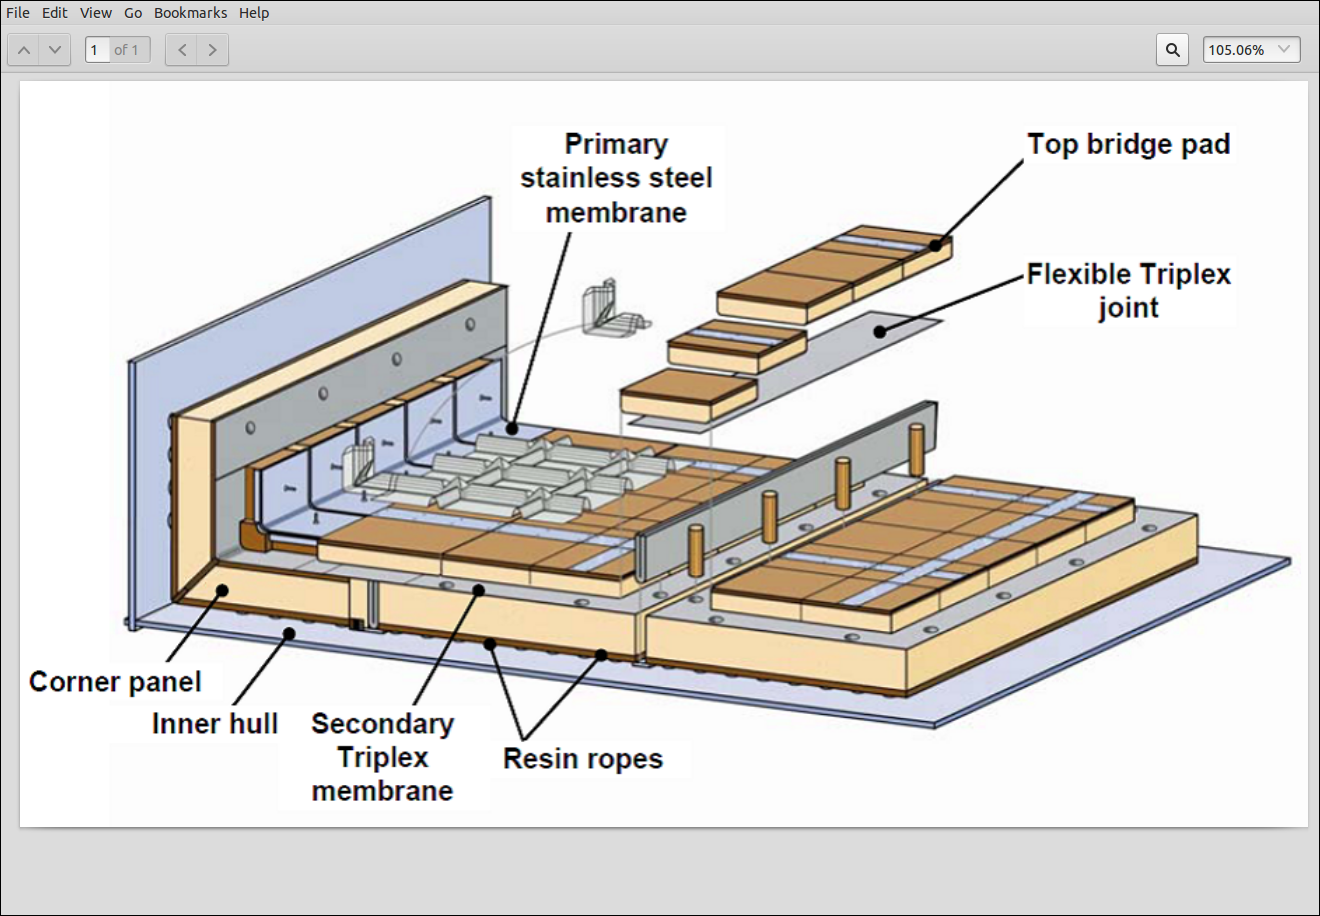
\includegraphics[width=.85\textwidth]{v5ch2-vessel-corner}
\caption{Membrane corner detail}
\label{fig:vessel-corner} %fig from email from russ 10/25
\end{figure}

The secondary membrane is comprised of a thin aluminum sheet and 
fiberglass cloth. The fiberglass-aluminum-fiberglass composite is 
very durable and flexible with an overall thickness of $\sim$1~mm.  
The secondary membrane is placed within the insulation space. It 
surrounds the internal tank on the bottom and sides, and it 
separates the insulation space into two distinct, leak-tight, 
inner and outer volumes. The outer insulation separates this 
membrane from the steel frame. This secondary membrane is connected 
to embedded metal plates in the vertical steel wall at the upper 
edge of the tank. In the unlikely event of an internal leak from 
the cryostat's primary membrane into the inner insulation space, 
the liquid cryogen will be contained in the 
secondary membrane volume.  

\section{Cryostat Layers as Packaged Units}
Membrane tank vendors have a ``cryostat in a kit'' design that 
incorporates insulation and secondary barriers into packaged 
units. See Figure~\ref{fig:gst-composite}.  
Figure~\ref{fig:composite-sys-install} illustrates how these 
layers would be used in the LBNF reference design.

\begin{figure}[htbp]
\centering
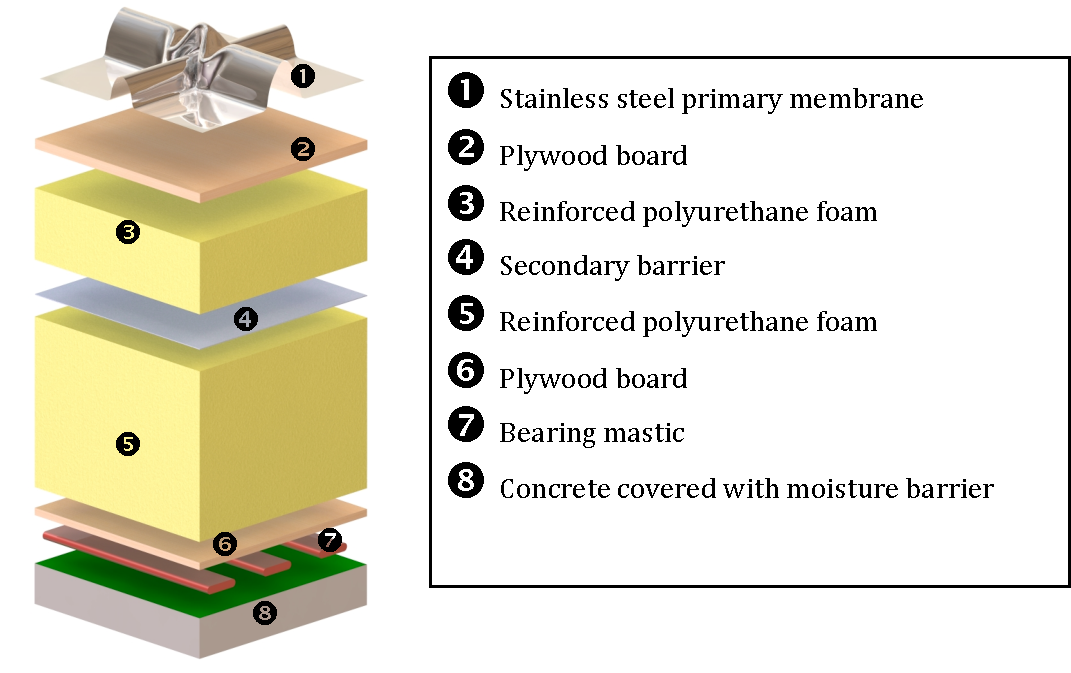
\includegraphics[width=0.8\textwidth]{v5ch2-gst-composite}
\caption{GST composite system from GTT}
\label{fig:gst-composite}
\end{figure}

\section{Top of Cryostat}

The stainless-steel primary membrane and the intermediate layers of 
insulation and water-vapor barrier continue across the top of the 
cryostat, providing a vapor-tight seal.  Note that no secondary 
membrane is required for the cryostat top. 

The hydrostatic load of the LAr in the cryostat is carried by 
the steel frame on the sides and bottom. Everything 
else within the cryostat (TPC planes, electronics, sensors,
cryogenic and gas connections) is supported by the top of the 
cryostat. All piping and electrical penetrations into the 
interior of the cryostat (except for sidewall penetrations from
the external liquid argon recirculation pumps) are made through 
this top plate to minimize the potential for leaks.

Studs are welded to the underside of the steel plates to bolt the 
insulation panels to the steel plates. Insulation plugs are inserted 
into the bolt-access holes.  The primary membrane panels (also 
manufactured in smaller sheets) are first tack-welded then fully 
welded to complete the inner cryostat volume. Feed-through 
ports located at regular intervals within the corrugation pattern
of the primary membrane to accommodate TPC hangers, electrical 
and fiber-optic cables, and piping are
shown in Figure~\ref{fig:v5ch2-roof-nozzle}. 

Some equipment, such as monitoring instrumentation, 
will be installed within wells extending through the roof 
structure. All connections into the cryostat (except for 
sidewall penetrations from the external liquid argon 
recirculation pumps) will be made 
via nozzles or penetrations above the maximum liquid level 
and mostly located on the roof of the cryostat. See figure 
\ref{fig:v5ch2-roof-nozzle} for a typical roof-port 
penetration.  

\begin{figure}[htbp]
\centering
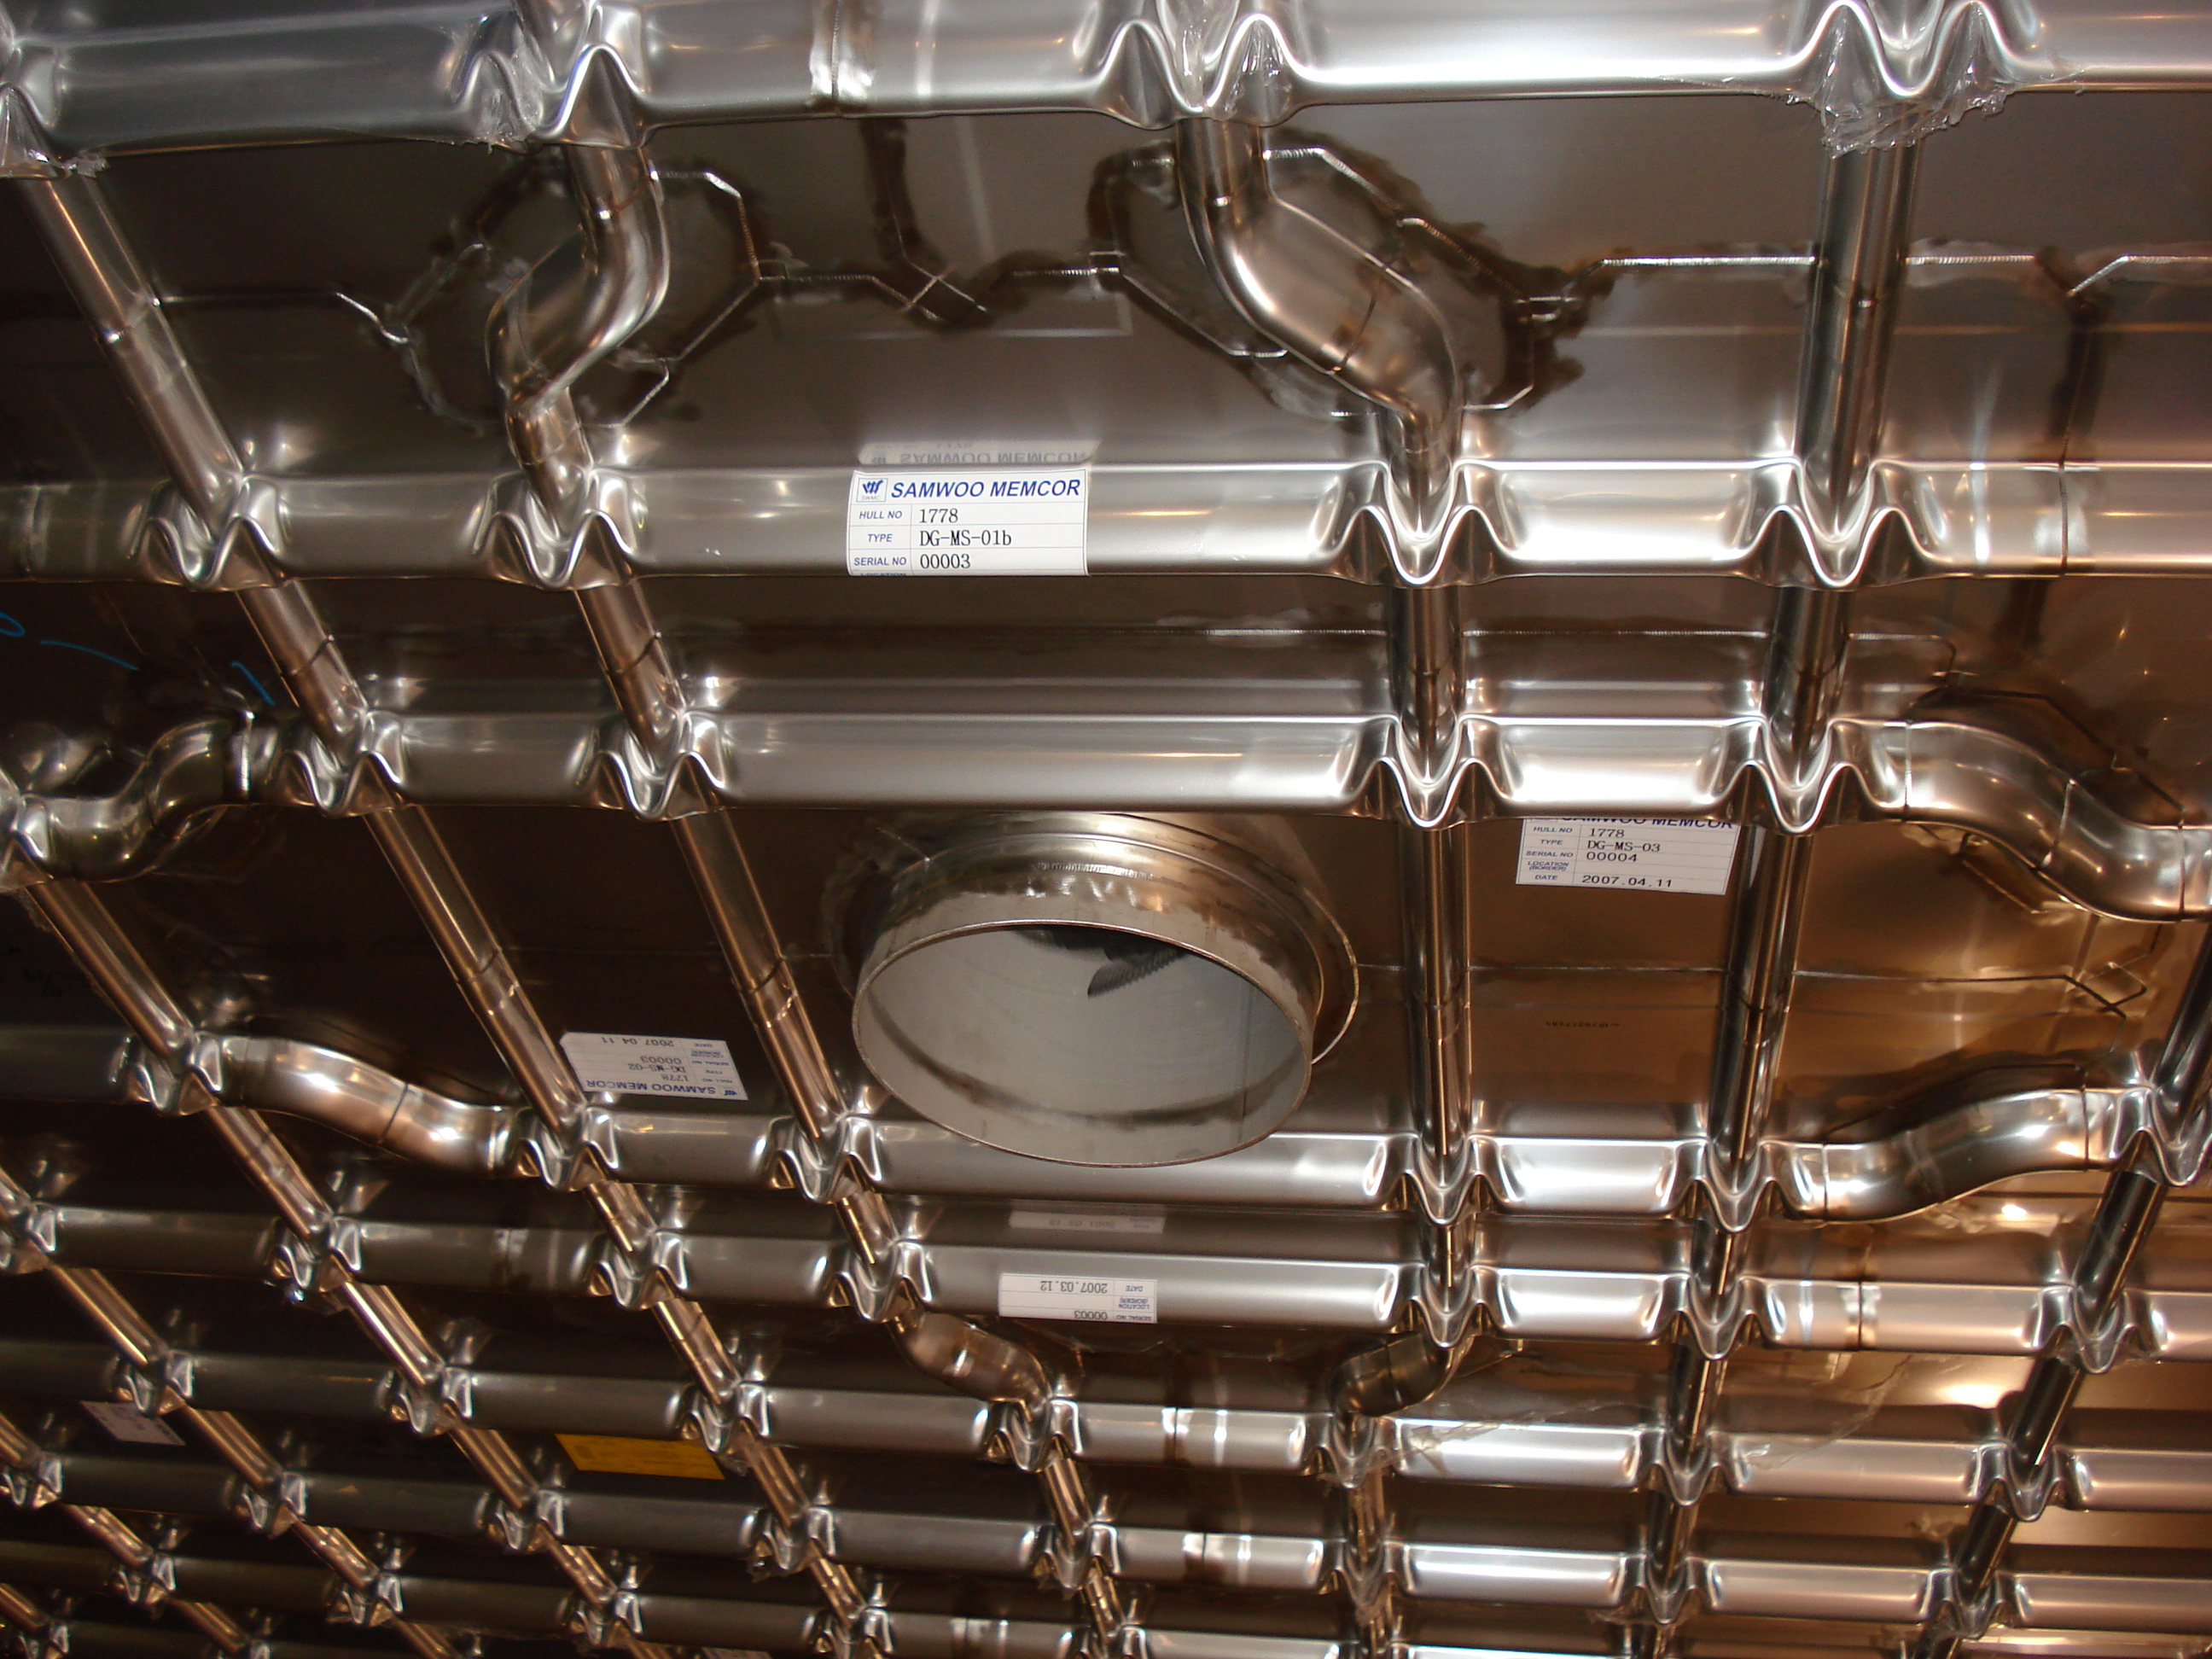
\includegraphics[width=0.45\textwidth]{v5ch2-roof-nozzle} 
\caption[Nozzles in the roof of membrane cryostat]{Nozzles in the roof of membrane cryostat (Figure courtesy GTT)}
\label{fig:v5ch2-roof-nozzle}
\end{figure}


\chapter{Leak Prevention}
\label{sec:cryo-cryosys-leak}

The primary membrane will be subjected to several leak tests 
and weld remediation, as necessary. All (100\%) of the welds 
will be tested by an Ammonia Colorimetric Leak Test (ASTM E1066-95) 
in which welds are painted with a reactive yellow paint before 
injecting gas with 25\% ammonia into the bottom insulation space 
of the cryostat.  Wherever the paint turns purple or blue, a leak 
is present. Any and all leaks will be repaired. The test will last 
more than 20 hours per cryostat and is sensitive enough to 
detect defects down to 0.003~mm in size and to a 10$^{-7}$ 
std-cm$^3$/s leak rate (equivalent leak at standard pressure 
and temperature, 1~atm and 273~K). Both membrane cryostat 
manufucturers use this technique for certifying that 
a cryostat is leak-tight.

%\section{Insulation Purge system}

To prevent infiltration of water-vapor or oxygen through 
microscopic membrane leaks (below detection level) the 
insulation spaces will be continuously purged to provide 
one volume exchange per day.  

The insulation space between the primary and 
secondary barriers will be maintained at 15 mbarg,  
slightly above atmospheric pressure. This space will
be monitored for changes that might indicate a leak 
from the primary membrane.  The outer insulation space 
will also be purged with argon at a slightly different 
pressure. The pressure gradient across the membrane walls 
will be maintained in the outward direction. Pressure-control 
devices and relief valves will be installed on both insulation 
spaces to ensure that the pressures in those spaces do not 
exceed the operating pressure inside the cryostat. 

The purge gas will be recirculated by a blower to a small 
purge gas dryer and reused as purge gas. The purge system 
is not safety-critical, and an outage of the blower would 
have only a minimal, short-term impact on operations~\cite{docdb4303}.

%%%%%%%%%%%%%%%%%%%%%%%%%%%%%%%%%%%%%%%%%%%%%%%%%%%%%%%%
\chapter{Cryogenic System Layout}
\label{sec:cryo-cryosys-layout}

Cryogenic system components are located in and around the surface 
building, in the Ross shaft and within the underground caverns. 
Figure~\ref{fig:eqp-at-surface} illustrates 
the cryogenic system layout. On the surface near the Ross 
shaft there will be a cryogen 
receiving station. A 50 m$^3$ (69 tons of LAr capacity) 
vertical dewar will have two LAr truck connections 
to allow for receipt of LAr deliveries for the initial
filling period. This liquid argon dewar serves as a buffer volume 
to accept liquid argon at a pace of about 5 LAr trailers 
(18 tons per trailer) per day during the fill period. An analyzer
rack with instruments to check water, nitrogen and oxygen content 
of the trailers will also be located in the vicinity. A large 
280 kW vaporizer at the surface is used to vaporize the liquid
argon from the storage dewar and warm up the resulting gas to 
room temperature prior to the argon gas being 
transferred by uninsulated piping down the Ross shaft.

\begin{figure}[htbp]
\centering
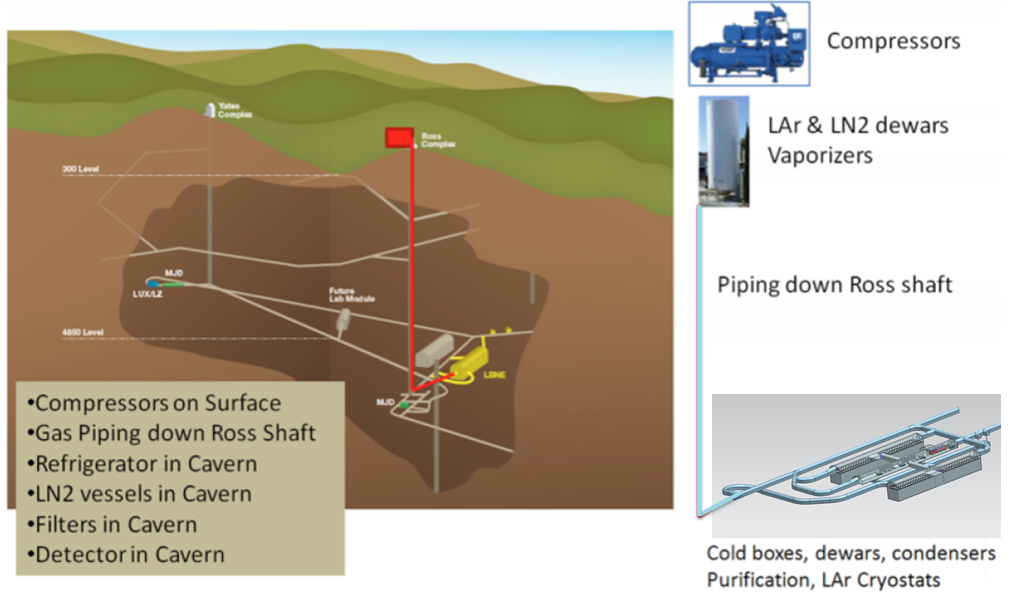
\includegraphics[width=\textwidth]{fd-cryosys-equip-location} 
\caption{Graphical illustrations showing major pieces of equipment and their location at the
surface, piping down the Ross shaft, and in the cavern area}
\label{fig:eqp-at-surface}
\end{figure}

Another 50 m$^3$ vertical dewar and fill connection will be 
available near the liquid argon dewar. This dewar is used 
to accept nitrogen deliveries for the initial charging and startup of
the nitrogen refrigerator. It is also used for pressure control of 
the liquid argon storage dewar. A large vaporizer for the nitrogen 
circuit nearby converts liquid nitrogen to nitrogen gas and warm to
warm the gas to room temperature. This gas is used as the feed for
the compressors of the nitrogen refrigerator. Four compressors are 
located in a compressor building on the surface near the Ross shaft 
and cryogen receiving area. The compressors require a set of nitrogen 
gas buffers as to regulate the nitrogen compressor low and high 
pressure loop, a set of oil separators and coalescers to clean the 
nitrogen gas after the pressurization loop, and a closed-loop water 
cooling circuit. The closed loop water-cooling circuit has 
recirculation pumps in the compressor 
building and an evaporative cooling tower located outside 
near the vaporizers. The compressors are the only refrigeration-cycle 
components located on the surface. The compressors discharge high 
pressure (1.14 MPa) nitrogen gas into
pipes that run down the Ross shaft. 
The reason why compressors were chosen to be on the 
surface is the electrical power and cooling supply 
are much cheaper to provide at the surface rather 
than at deep depth in the mine. Each compressor is an 
1500 horsepower machine running at 4160 volts. 
Four running compressors will require a total of
2.6 MW of electrical power at the surface.


The Ross shaft contains the vertical pipelines connecting the 
surface equipment with the equipment in the cavern area. The 
vertical piping run is described in 
Chapter~\ref{sec:cryo-cryosys-pipework-surface-cav}. 
The piping run consists of a GAr transfer line and the 
GN$_2$ compressor suction and discharge lines. At the bottom of 
the Ross shaft at the 4850 level, the piping exits the 
shaft and runs along a drift to the cavern area.

The central utility cavern at the 4850 level contains the
rest of the nitrogen refrigerator (cold boxes), liquid
nitrogen storage vessels, and filtration equipment.
The nitrogen refrigerator equipment is located at the far
end of the central utility cavern, away from Ross shaft.
Fresh ventilation air is supplied down the Ross and Yates shafts, 
enters the detector caverns and flows over the cryostats 
or the refrigerator equipment in the central utility 
cavern before being exhausted out via the Oro Hondo
exhaust shaft.

There are four argon recondensers per cryostat. They are 
placed above each cryostat. Four 23 m$^3$/hr recirculation 
pumps per cryostat are used to circulate liquid from the bottom 
of the cryostat through the LAr filters and are set close to 
each cryostat as well. Each pump will have sidewall
penetration to the membrane cryostat. 


\chapter{Pipework between Surface and Cavern}
\label{sec:cryo-cryosys-pipework-surface-cav}

The effort on pipework between surface and cavern is divided among the
cryogenics infrastructure WBS and conventional facility (CF) WBS. The
conceptualization of the piping has been done as part of cryogenic
infrastructure, while the support system design as well as the
construction of these piping system shall be carried out by CF.

The piping between the surface and cavern area is located in a utility 
chase down the Ross shaft. See Figure~\ref{fig:framing-at-ross-piping}. 
The piping material is carbon steel coated with a corrosion barrier,
a single layer of fusion epoxy. Table~\ref{table:pipelines} lists 
the piping and its duty 
and size. The frictional pressure drop for the supply pipes matches
the pressure gained due to the static head from elevation change. 
All the piping connections will be made with victaulic fittings. 
The nitrogen and argon 
being transferred in the Ross shaft piping will be at ambient 
temperature, in the gas phase. Having gas phase only in the 
1.5 km vertical piping is an advantage over liquid transfer 
because the hydrostatic head for gas only piping is on the order of
0.05 MPa, whereas for the liquid transfer it is 20 MPa. If 
liquid was transferred it would require on the order of
seven pressure reducing stations evenly spaced along the vertical drop.
Using liquid cryogen delivery was considered in the March 
2012 LBNE CDR. However, the cost of providing 
the excavated spaces and pressure reducing stations was costly 
as compared to using gas only transfer. For a liquid transfer
option with pressure reducing stations, the piping would need 
to be routed down the Oro Hondo ventilation shaft which would 
need rehabilitation. With gas 
only transfer to the cavern, straight piping can be run down 
the Ross shaft. The drawback of gas only transfer is that one 
must provide the liquid nitrogen refrigeration in the cavern 
to fill the cryostats by liquid argon condensation. Filling 
each cryostat with liquid argon in a reasonable period of 
time is a driving factor to determine the size of the 
refrigerator and condenser.

\begin{table}
\caption{Piping between surface and cavern area; description, duty, 
and size and pressure required}
\label{table:pipelines}
\begin{tabular}[htbp]{|p{0.24\textwidth}|p{0.26\textwidth}|p{0.21\textwidth}|p{0.185\textwidth}|}
\hline
{\bf Description} & {\bf Duty} & {\bf [No. of Pipes] Size} & {\bf Gas Pressure} \\
\hline\hline
Argon transfer   & During filling and emptying & [1] 8'' SCH. 40  &  0.24 MPa\\
\hline
N$_2$ compressor discharge & Continuous & [2] 8'' SCH. 40 & 1.14 MPa \\
\hline
N$_2$ compressor suction & Continuous & [3] 12'' SCH. 40 & 0.19 MPa (down);  \\
                         &            &                        & 0.11 MPa (up) \\
\hline\end{tabular} 
\end{table}

The facility is designed that the fresh air is drawn
in through Ross and Yates shafts
%(100,000 cfm)
and the exhaust
air is drawn out of mine through Oro Hondo shaft.
%(290,000$-$500,000 cfm).
The loss of mine ventillation for more than a few hours risks mine safety
even without oxygen deficiency hazard (ODH) condition.
%The loss of ventillation
%could occur, when vent piping to exhaust shaft collapses due to
%rockfall or significant events causing major damage on the facility
%such as earthquakes (which are unlikely to happen in the
%lifetime of experiment).

A preliminary ODH assessment for 
the piping in the Ross shaft has been done. If any of the pipes
for the cryogenic system are ruptured in the shaft, they would
only be able to reduce the oxygen content to a fraction of 20.5\%, 
thus not being an oxygen deficiency concern. The ODH mapping
of underground cavern area is given in Chapter~\ref{sec:cryo-cryosys-esh}.

\begin{figure}[htbp]
\centering
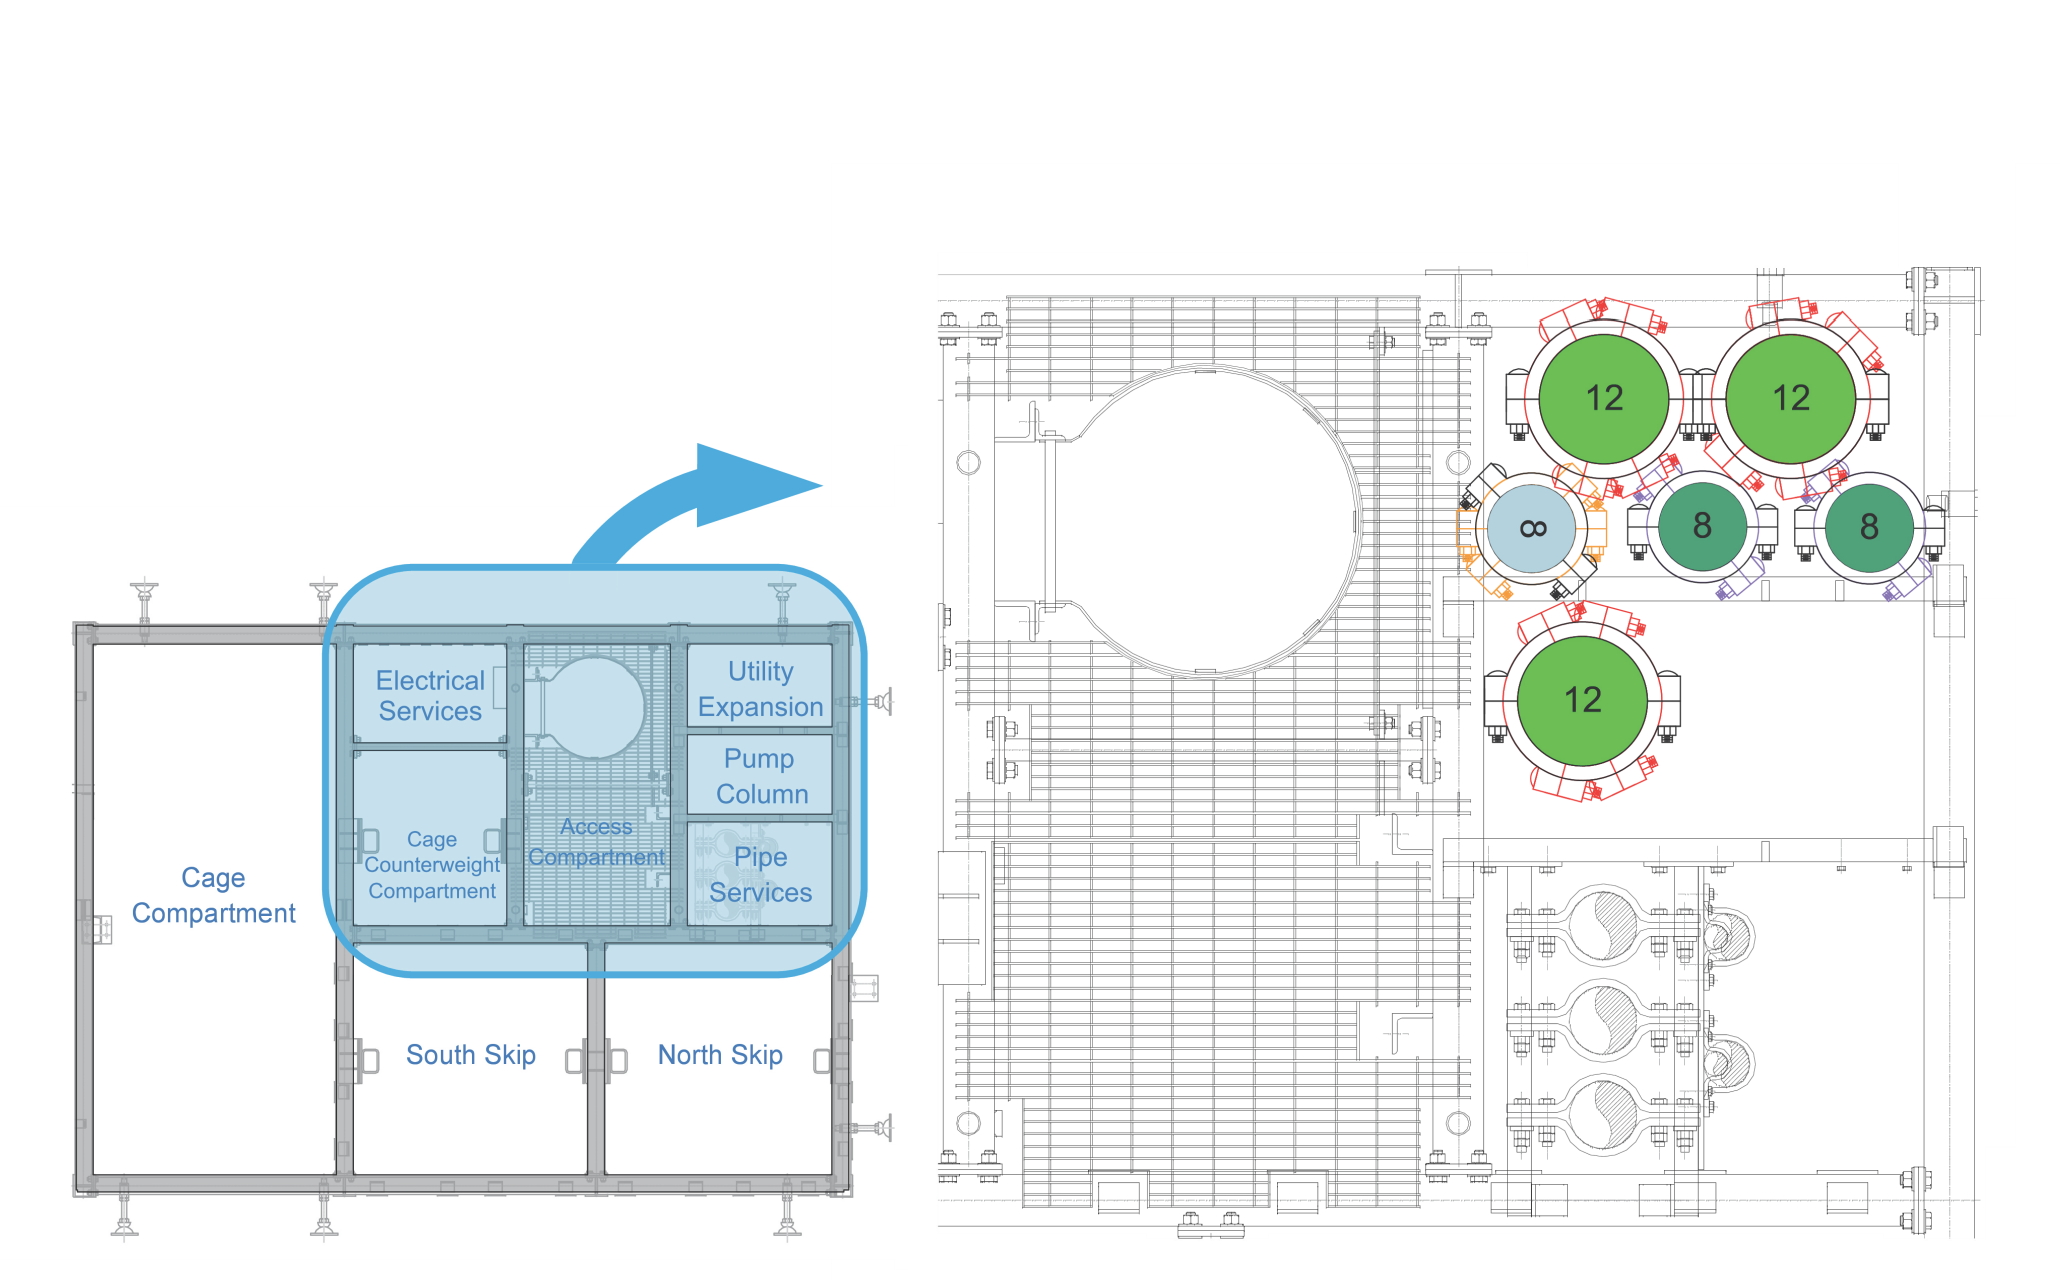
\includegraphics[width=\textwidth]{ross-shaft-pipes.png} 
\caption{The framing of the Ross shaft is shown on the left. The utility area in the upper
right corner contains the piping
associated with the cryogenic system.}
\label{fig:framing-at-ross-piping}
\end{figure}

\begin{figure}[htbp]
\centering
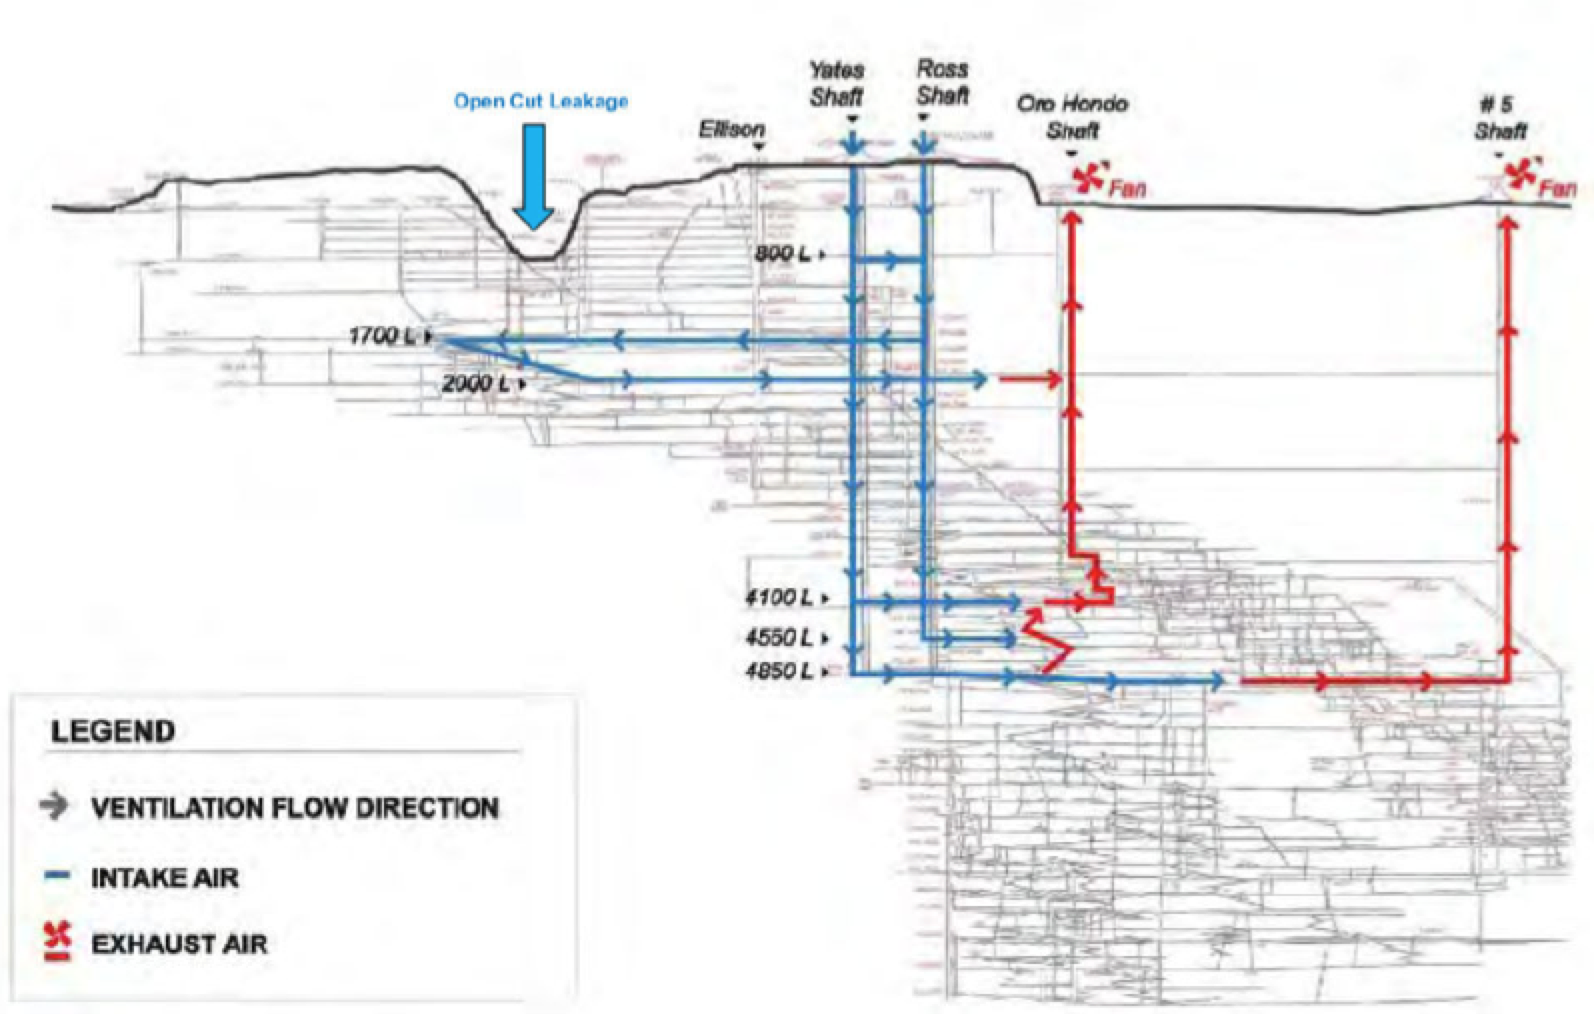
\includegraphics[width=\textwidth]{homestake-ventilation-paths.png} 
\caption{Homestake mine ventilation paths}
\label{fig:ventilation-paths}
\end{figure}

\chapter{Equipment in the Cavern Area}
\label{sec:cryo-cryosys-equip-cavern}

There are four independent 85 kW (maximum capacity: 20\% up above nominal) 
nitrogen refrigerators in the central utility cavern. The nitrogen
refrigerator heat exchangers and expander sets are located 
at the east end of the central utility cavern.
The heat exchangers (1.2 m diameter $\times$ 9.1 m long) 
will be in a horizontal orientation in order to
fit them within the cavern. The liquid nitrogen produced 
by the refrigerators is stored in six horizontal 
8.3 m$^3$ (1.2 m diameter $\times$ 11 m long) liquid 
nitrogen vessels per cryostat that are mounted in the
central utility cavern. These liquid nitrogen vessels
feed the argon condensers that are connected 
to the cryostat. The returning nitrogen gas from the 
condensers is routed through the refrigerator heat 
exchangers and warmed to ambient temperature. The 
nitrogen gas is then boosted by four independent 120 kW 
compressors located in the central utility cavern to 0.19 MPa 
and returned in the nitrogen suction piping 
in the Ross shaft.

Four argon condensers (0.8 m diameter $\times$ 2.0 m long) 
are located above each of the cryostats. The full 
power of the argon condensers is used during the initial 
cooldown and filling phase of the cryostats in order to
condense the gas argon transferred down the Ross 
shaft. The fill process is expected to take between 6 and 16 months. 
The fill time durations given here assume three refrigeration 
units available for the first and second cryostat fill and
all four units available for the third and fourth cryostats (where
steady state operations are maintaining liquid in the full cryostats).
Additional information about the filling process is 
described in Chapter~\ref{sec:cryo-cryosys-proc}.  

%\begin{editornote}
%  Editor's Note:  Filling times in preceding sentences refer to filling two 17-kton modules.
%\end{editornote}


Purification filters are located in the central utility cavern 
as shown in Figure~\ref{fig:det-cavern-purif}. The filters (1.0 m
diameter $\times$ 4.3 m high) contain dual media, a molecular 
sieve for removal of water and a copper coated catalyst media 
for oxygen removal. There are four gas filters used during 
the argon filling phase and four liquid filters for each cryostat. 
Associated with the filters, there will be regeneration 
equipment such as heaters, gas blowers, and a hydrogen
generator also located in the central utility cavern.

\begin{figure}[htbp]
\centering
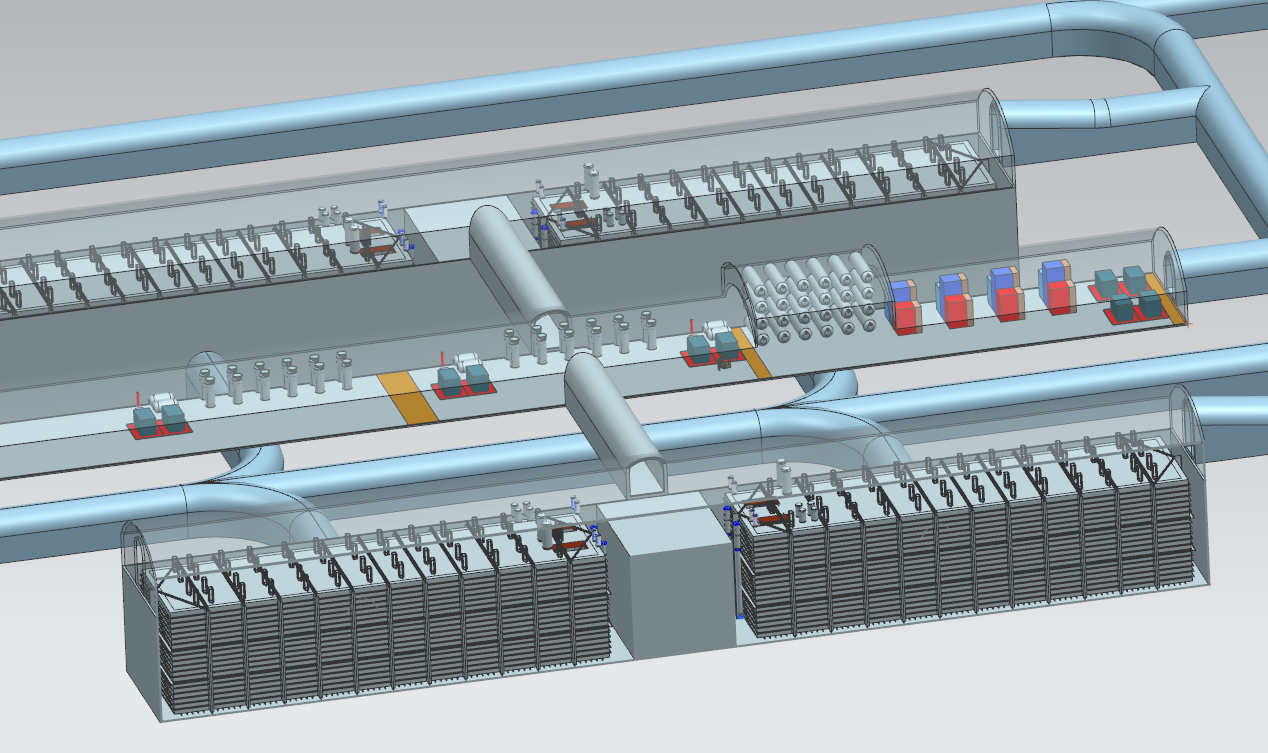
\includegraphics[width=\textwidth]{DUNE-FD.png} 
\caption{Isometric view of the underground caverns (not to scale)}
\label{fig:det-cavern-purif}
\end{figure}


\chapter{Cryogenic System Process}
\label{sec:cryo-cryosys-proc}
%added by russ 10/6
The entire cryogenic system process is summarized with functions of 
every cryogenic system component in 
Figure~\ref{fig:v5ch2-LBNF-block-diagram-2014}.  
The major functions serving the cryostat are cryogen supply for 
cooldown and fill, gas filtration, argon condensing, liquid 
circulation and filtration, and argon-purity analysis. 
The methods presented in this section are motivated by
experience from the cryogenic systems of other LArTPC 
experiments, such as ICARUS, LAPD and prototype 35 ton 
membrane cryostat. The piping
connections between major cryogenic system components 
are shown in Figure~\ref{fig:v5ch2-LBNF-cryo-process-2014}.

\section{Cryostat Inital Purge and Cool-down}

After cryostat construction and following installation of all 
scientific equipment, the cryostat will be cleaned, purged and 
cooled. Construction procedures leading up to this point will
ensure that the completed cryostat does not contain debris and is free
of all loose material that may contaminate the LAr.

\subsection{Initial Purge} 

Argon piping will be isolated, evacuated to less than 0.1 mbar
absolute pressure and backfilled with high-purity argon gas.
This cycle will be repeated several times to reduce contamination
levels in the piping to the ppm level. The reference-design choice
for removing air from the membrane cryostat is argon
flow/piston-purge, introducing the heavier argon gas at the
bottom of the cryostat and removing the exhaust at the top. The bottom
field cage (part of the TPC) serves an additional role as a flow
diffuser during the initial purge. A matrix of small holes in the
field cage, approximately 10 mm diameter at a 50 mm pitch,
will provide a uniform flow.

The flow velocity of the advancing argon-gas volume will be set to 1.2 m/hour.
This velocity is high enough to efficiently overcome the molecular diffusion
of the air downward into the advancing argon so that the advancing pure
argon-gas wave front will displace the air rather than just dilute it.
A 2D Computational Fluid Dynamics (CFD) simulation of the purge process
on the 5 kton fiducial-mass cryostat for LBNE shows that after 20 hours
of purge time, and 1.5 volume changes, the air concentration will be
reduced to less than 1\%. At 40 hours of elapsed time and three volume
changes, the purge process is complete with residual air reduced to a
few ppm. This simulation includes a representation of the perforated
field cage at the top and bottom of the detector.  The cathode planes
are modeled as non-porous plates although they will actually be
constructed of stainless-steel mesh.

The computational fluid dynamics (CFD) model of the purge process 
has been verified in multiple arrangements: (1) in an instrumented 
cylinder of 1 m diameter by 2 m height, (2) Liquid Argon Purity 
Demonstrator (LAPD), a vertical cylindrical tank of 3 m diameter by 3 m height,
taking gas-sampling measurements at varying heights and times during 
the purge process, (3) within the 35 ton membrane cryostat, a 
prototype vessel built for LBNE in 2013, of which the results 
are found at~\cite{Montanari:2013/06/13aqa}, % used label from inspirehep {35ton-prototype}. 
and (4) within MicroBooNE cryostat, a horizontal cylindrical
tank of 3.8 m diameter by 12.2 m length.

\begin{figure}[htbp]
\centering
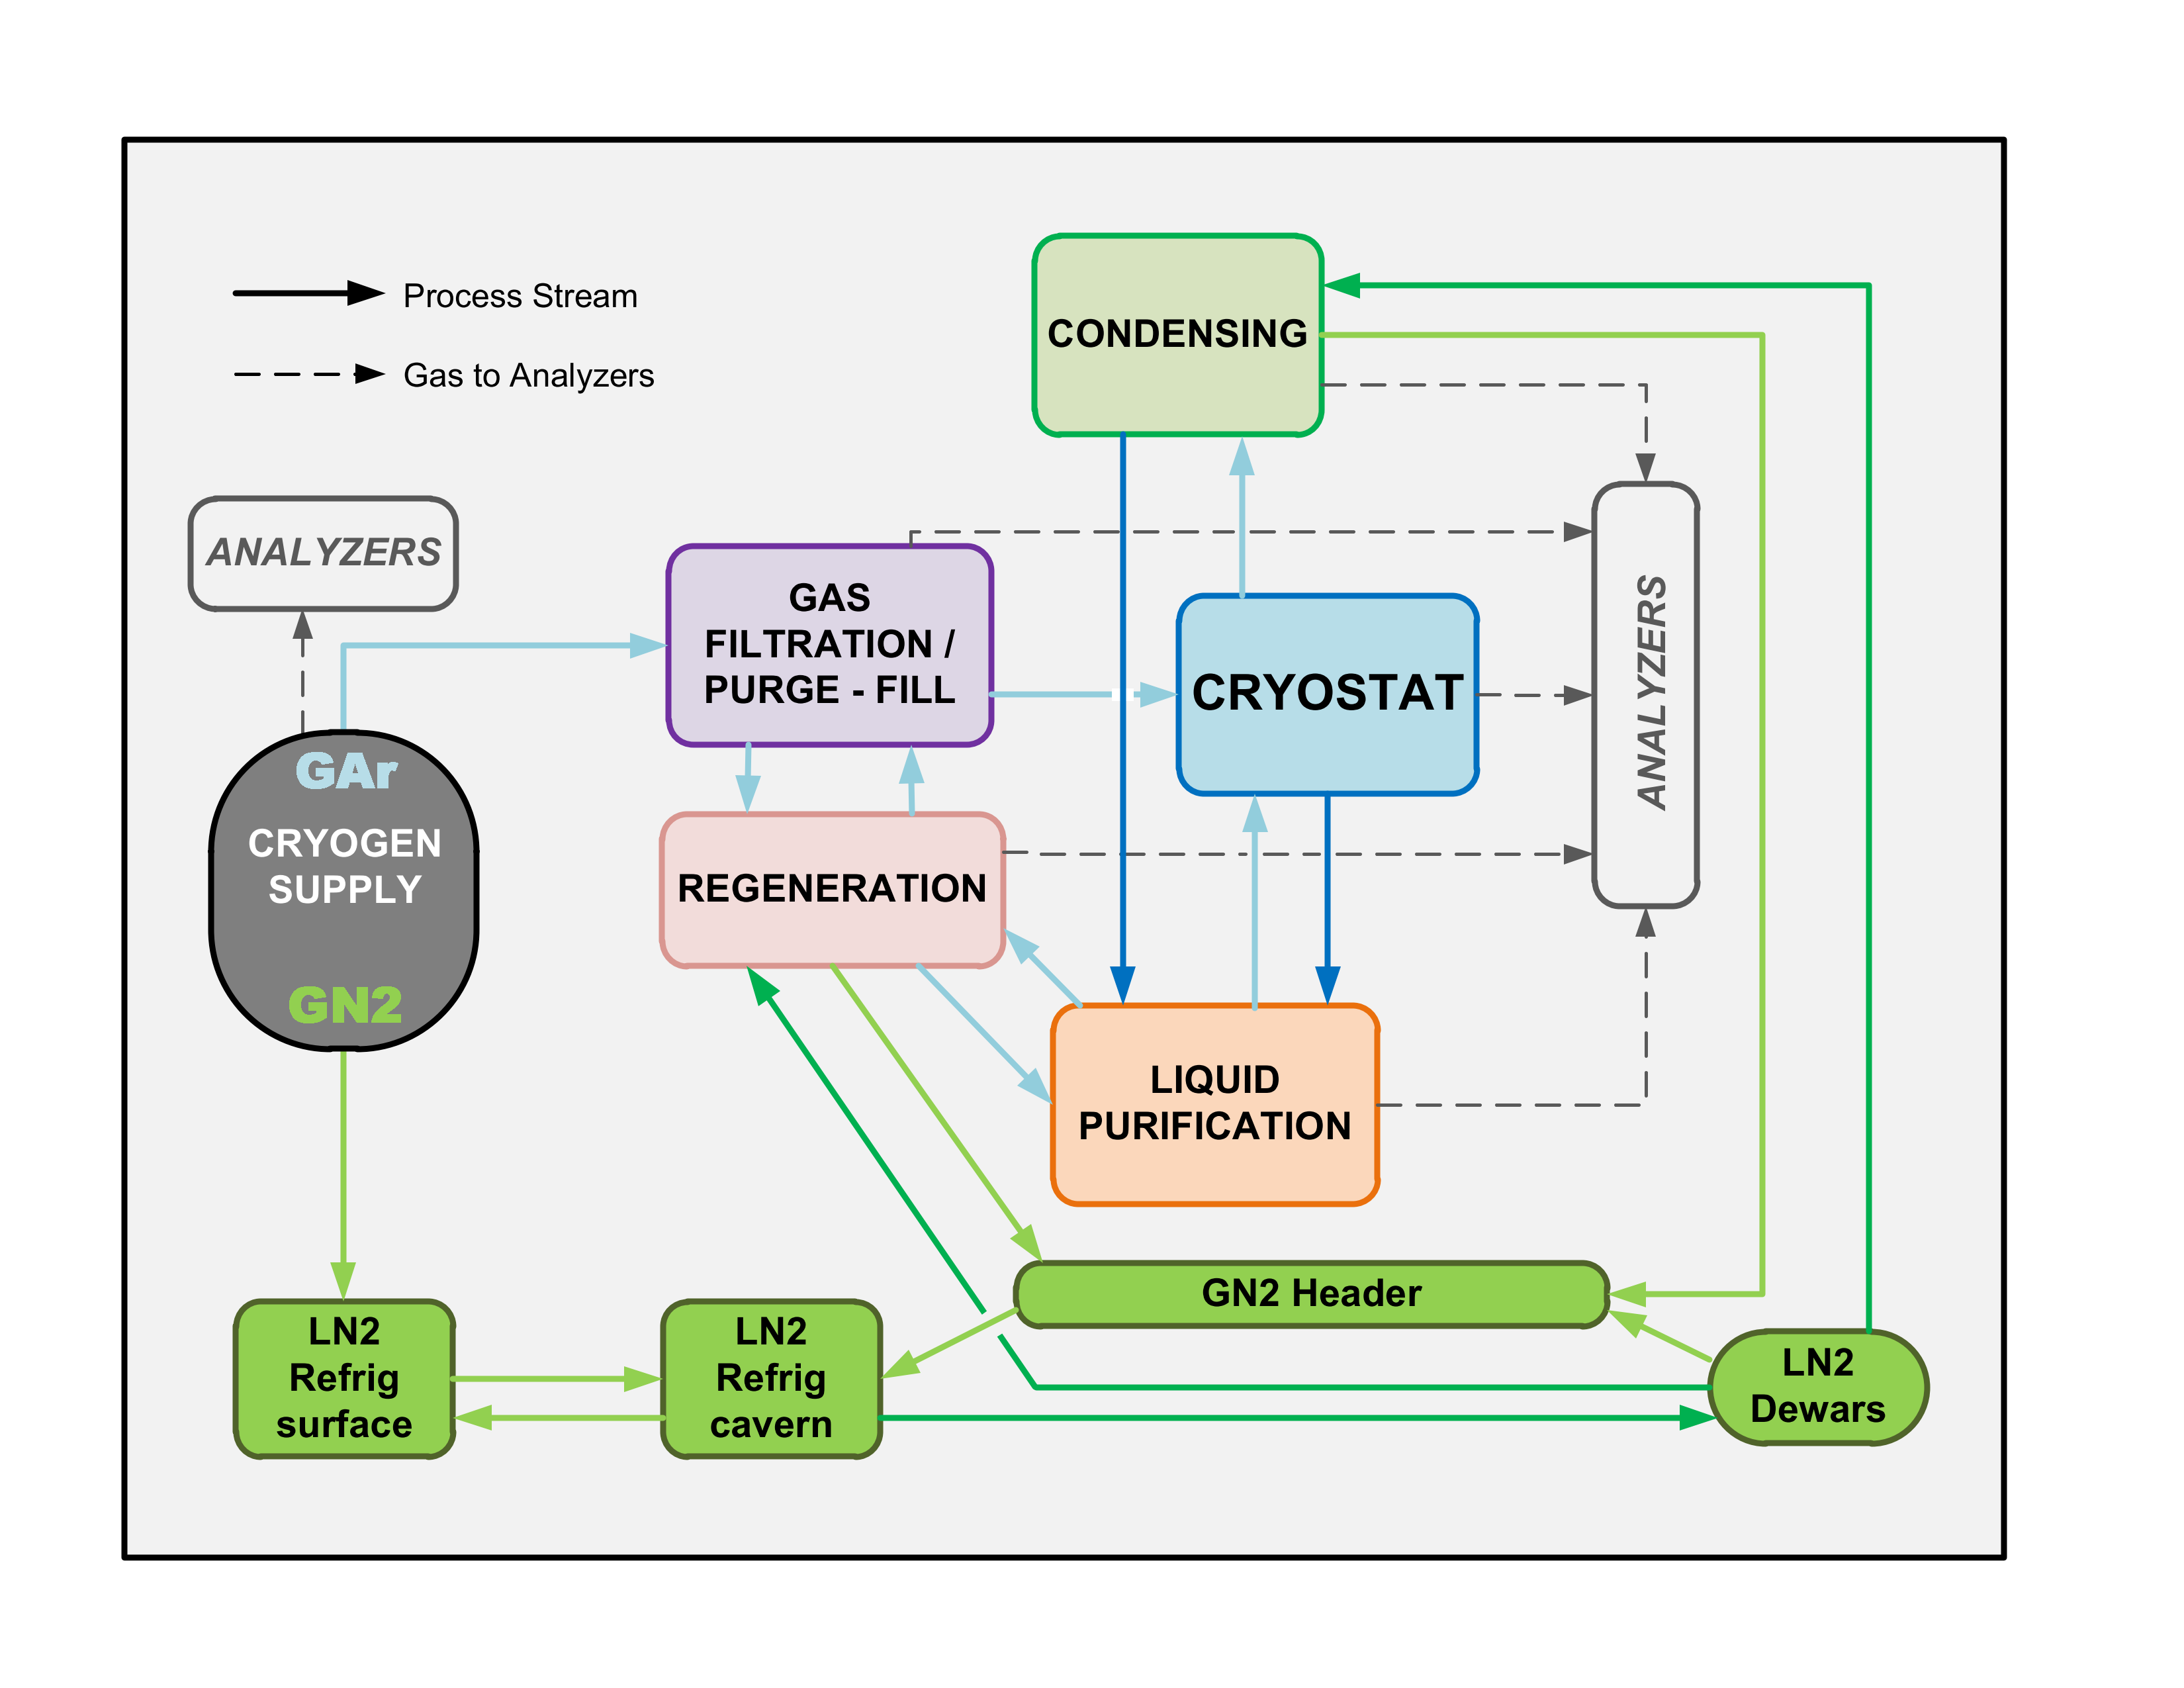
\includegraphics[width=1.05\textwidth]{cryosys-functions.png} 
\caption{Cryogenic system functions}
\label{fig:v5ch2-LBNF-block-diagram-2014}
\end{figure}

\begin{figure}[htbp]
\centering
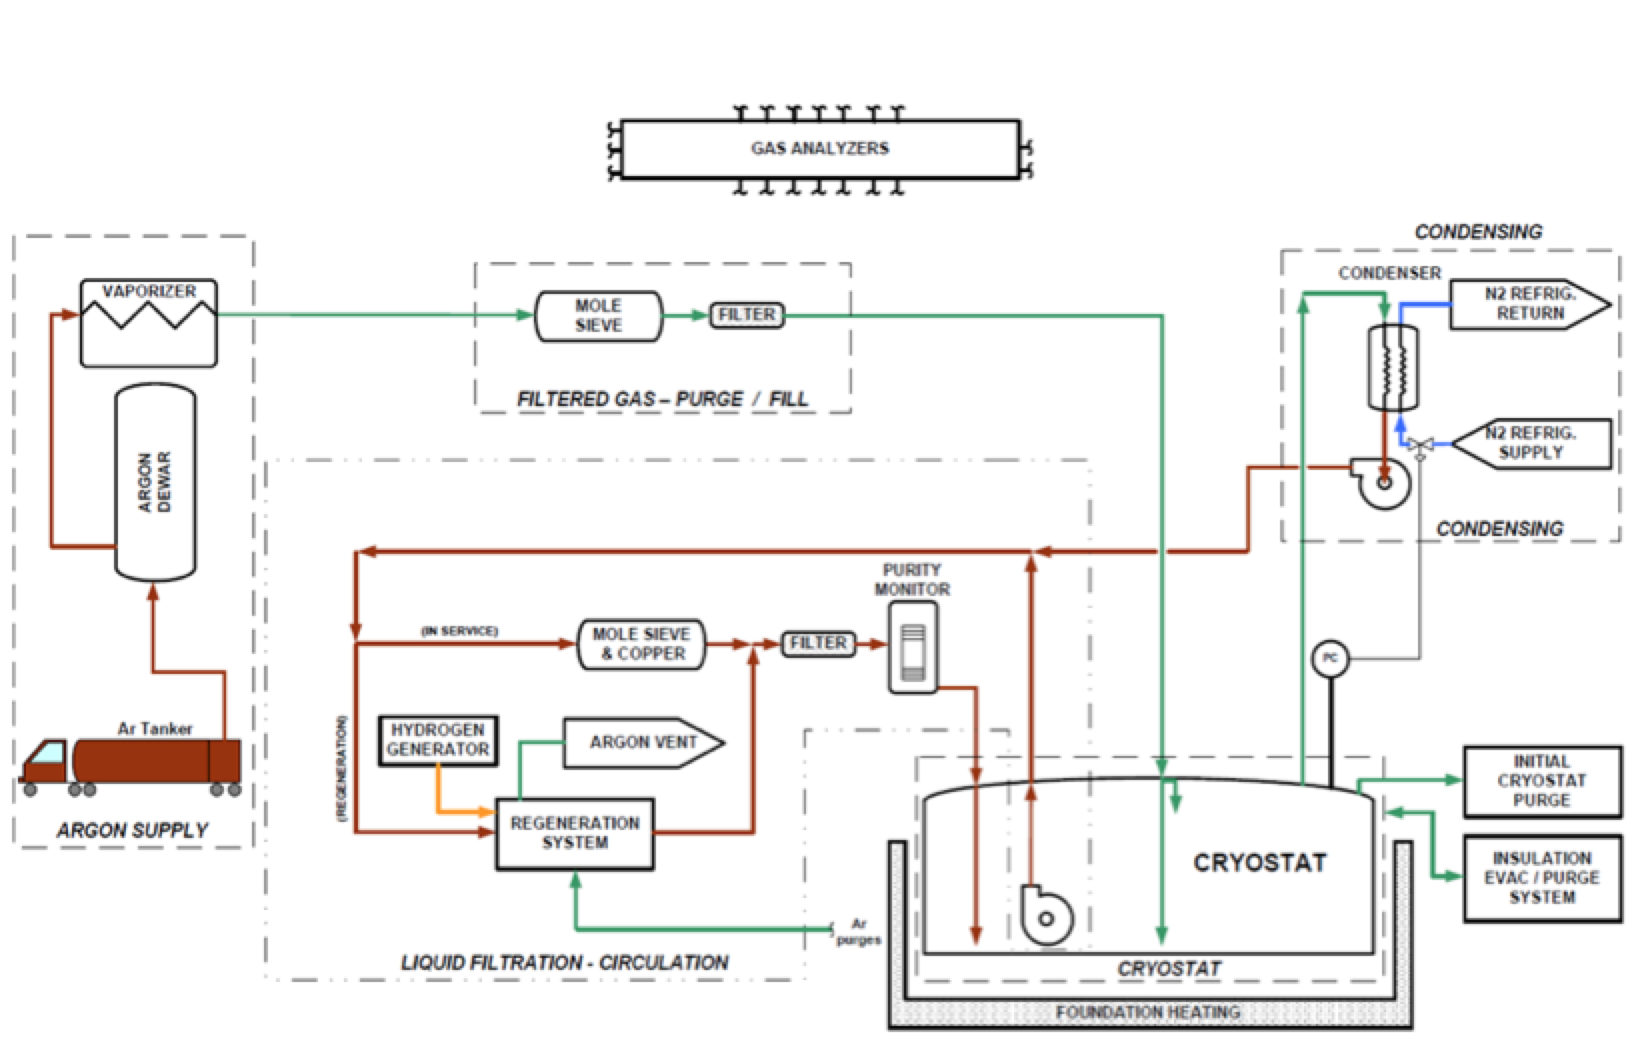
\includegraphics[width=1.25\textwidth,angle=90]{cryosys-flow.png} 
\caption{Cryogenic system flow block diagram}
\label{fig:v5ch2-LBNF-cryo-process-2014}
\end{figure}


% The elements of the plan and their applicability to LBNF are described in Chapter~\ref{ch:randd}.  BN didn't think this fit for techical report 10/06/11

\subsection{Water Removal via Gas Flow}

Water and oxygen will be removed continuously from the system for several days following the
initial purge. Flowing gas will be used at the same rate, however at this stage the gas will
be filtered and recirculated. Each cryostat contains five tons of FR4
circuit-board material and a
smaller inventory of plastic-jacketed power and signal cables. These somewhat porous
materials may contain as much as 0.5\% water by weight. Water-vapor outgassing from these
materials will be entrained in the gas flow exiting
the top of the cryostat and will be removed
from the gas stream by filters. Adsorbed water will also be removed from the metallic inner
surfaces of the cryostat and piping system. Water deep within porous materials will remain;
this is not a problem since
the water diffusion rate in FR4 at room temperature is already 
quite low (0.3~$\mu m^2 /s$) and the FR4 assemblies are relatively thick (1~cm).

%\subsection{Alternative Water-Removal Method: Evacuation}

%Another method for removing water and oxygen from LArTPC experiments 
%is to evacuate the tank to $\sim$10$^{-4}$~mbar  and then backfill it with 
%pure argon gas. Although the primary membrane of the reference-design 
%cryostat is not a vacuum vessel, it is possible to evacuate it.
%Membrane-cryostat vendors report that evacuation of  the insulation 
%spaces (external to the primary membrane) is normally done during the 
%construction and leak-checking phases.  A vacuum pressure of less than 
%200~mbar absolute in the insulation spaces has so far been achieved. 
%As long as the pressure-differential direction across the walls is 
%kept outward, it is possible to reduce the internal membrane-tank 
%volume to these pressures as well.  

\subsection{Initial Cool-Down}

Purified LAr will be distributed near
the bottom of the cryostat to cool down the cryostat in a controlled spray.
The boil-off gas will flow through the volume of the cryostat, then
routed to the recondenser and liquid-filtration system. Simulation
has shown that the liquid cool-down method can
be controlled to stay within the available recondenser capacity. The required cooling rate
is determined by the maximum stress that DUNE detector components can
tolerate. For example, the 150 $\mu$m APA wires will cool much more rapidly than the APA frames.
A mass flow control system with temperature-monitoring system will be used to control the
temperature difference across the cryostat. The exact temperature difference required is yet to
be determined; it will be based on input from the cryostat designer and the restrictions from
the TPC components and structure.

\subsection{Initial Purge and Cool-Down Design Features}

Internal piping is positioned within the cryostat to support the purge and cool-down procedure.  Heavy argon vapor, which is a result of cooling down the membrane bottom with liquid, will promote purging after it rises from the base of the cryostat and is vented from the roof level.  The LAr-supply pipework will have nozzles spaced along its length to 
 distribute equal liquid-delivery flow rates across the bottom of the cryostat.  The flow nozzles will be directed downward or to the side so that the injection velocity will not cause local vertical gas plumes or turbulent mixing but rather will spread across the bottom of the cryostat and produce a stable, upwardly advancing argon wave front. The vertical velocity of 1.2~m/hr for the gas purge includes a contingency for some level of turbulent mixing. 

Main gas returns, used for pressure control, will be distributed along the cryostat roof.  All nozzles and dead-end (stagnant) volumes located at the top of the cryostat will have gas-exhaust lines for the initial purge and for continuous sweep-purge of those volumes during normal operations.  
The sweep-purge during the initial stage of purging will be vented outside of the cavern.  After all but trace amounts of air have been expelled, the gas returns will be routed to the recondensers before being returned to the cryostat.  When cool-down to 120~K is complete (and during steady state operations), the gas returns will be sent to the recondenser to be liquefied by heat exchange with a liquid nitrogen stream.  The recondensed liquid will be filtered and sent back to the cryostat to complete the cool-down operation.
All purge gas will be either vented outside of the cavern at a remote location, or recondensed and reused. 

\section{Liquid Argon Receipt}

Each 10 kton fiducial mass membrane cryostat will hold an inventory 
of 17.1~kton of liquid argon. Considering that some quantities will 
be lost in transit, as a start (17.1+$\alpha$) kton of LAr will need to be 
procured to fill the first cryostat. Planning the supply and logistics 
of LAr delivery to the facility requires consideration of the following issues:

\begin{itemize}
\item  Total capacity of commercial air-separation plants within freight 
distance of the facility (the peak delivery potential)
\item Extent of boil-off that will occur in transit (that is the biggest 
contribution to determine $\alpha$)
\item Number of vehicle movements required and their impact on the local community
\item Costs and benefits associated with stockpiling LAr at the facility
ahead of commencing the purge, cool-down and fill procedure
\item Provision of a temporary air-separation plant at the facility 
to generate liquid argon
\item Availability and cost associated with the delivery of high-purity 
LAr as opposed to lower-quality commercial-grade argon combined with 
on-site coarse purification
\end{itemize}

The current total argon capacity in the United States is approximately 5.2 kton/day, 
whereas the demand is about 4.7 kton/day, which means 90\% capacity utilization in 
2015. Argon demand slowed down during recession (2008$-$2009), but has been 
recovering strongly since 2010, especially in electronics and welding industries, 
in a pace faster than capacity growth. Some capacity was taken offline in recession 
and has not come back. The trend of growing demand at a rate of 3.4\% per year, 
faster than capacity, is expected to continue for at least the next five years and 
will cause argon supply to be tight and prices to rise. Therefore, creating clusters 
of existing argon capacity that can provide argon to LBNF, rather than using one 
supplier, or identifying new argon capacity (preferrably closer to SURF site) can 
be options to consider for economic and reliable supply. At the time of market 
research, air separation plants (ASPs) in Chicago and the Gulf Coast were 
identified as the most important supply source, but this option will 
require significant delivery cost.

The standard grade specification for argon is a minimum purity of
 99.995\%, allowing a maximum concentration of 5.0~ppm for O$_2$ 
and 10.5~ppm for H$_{2}$O.  This is designated as Grade 4.5 in 
the gas-supply industry.  Requiring higher-purity product would 
significantly reduce the volume of product available to the 
experiment, increasing cost and pushing out the schedule.  
Therefore, it is likely that standard product will be 
procured from multiple vendors.  

The most efficient mode of argon delivery seems to be
over-the-road tank truck with a maximum capacity of 18.7~metric ton (MT).  
The expected number of such deliveries per cryostat is about 1000 
over six to sixteen months (Find more details in 
Chapter \ref{sec:cryo-cryosys-equip-cavern} and Section 
\ref{sec:refrigeration-load-scenarios}). 
Rail delivery is not cost-effective as there are no rail spurs leading
to the SURF site. This mode would require transfer of product from rail 
tanker to a tank truck, introducing cost that exceeds the benefit.

Surface facilities for offloading LN$_{2}$ and LAr road tankers are 
required. It will be necessary to  procure approximately four trailer 
loads of liquid nitrogen (about 40~tons) for the initial filling of 
the LN$_{2}$ refrigeration dewar and charging of a single refrigeration 
plant. Vehicle access and hard-surfaced driving areas are required 
adjacent to the LN$_{2}$ and LAr dewars. An interim 
LAr storage dewar will hold the contents of a few road tankers in order 
to minimize off-loading time.  Road tankers will connect to a 
manifold and will use their on-board pumps to transfer the LAr 
to the storage dewar. Each tanker will be tested to ensure that 
the LAr meets the purity specification. The LAr will be 
stored in the surface dewar and vaporized before transporting 
by pipe feed to the underground cavern for liquefaction.

\section{Cryostat Filling}

Liquid argon will be delivered to the cryostat through the 
cryostat-filling pipework. Argon will be piped to the cavern 
in gas form from the surface and condensed/liquefied via the 
LN$_{2}$ exchange in the condenser units. The filling process 
will take place over many months due to the delivery schedule 
of liquid argon described in the previous section and the 
need to condense gaseous argon. Liquid-argon purification 
can begin once the liquid depth reaches about 2 m in the cryostat. 
At this depth, the recirculation pumps can be safely
turned on and it will direct up to 93~m$^{3}$/hr (411~gpm) 
of liquid argon through the purification system.

\section{Argon Reliquefaction and Pressure Control}
\label{subsec:reliquef}

The high-purity liquid argon stored in the cryostat will 
continuously evaporate due to the unavoidable heat ingress.  
The argon vapor (boil-off gas) will be recovered, chilled, 
recondensed and returned to the cryostat. A closed system 
is required in order to prevent the loss of the high-purity argon.

During normal operation the expected heat ingress of approximately 
69.9 kW to the argon system will result in 
an evaporation rate of 1571 kg/hr and expanding in volume by a 
factor of 200 when it changes from the liquid to vapor phase. 
This increase in volume within a closed system will, in the 
absence of a pressure-control system, raise the internal pressure.

In LBNF, argon vapor will be removed from the top of the cryostat 
through the chimneys that contain the cryogenic feedthroughs. As 
the vapor rises, it cools the cables and feedthrough, thereby 
minimizing the outgassing. The exiting gaseous argon will be 
directed to a heat exchanger (a recondenser, illustrated in 
Figure~\ref{fig:v5ch2-recondenser-sept-2011}) in which it is 
chilled against a stream of liquid nitrogen and condensed 
back to a liquid. As the argon vapor cools, its volume 
reduces and in the absence of pressure control further 
gas would be drawn into the heat exchanger, developing 
a thermal siphon.  Therefore, a pressure-control valve on 
the boil-off gas lines will control the flow to the recondenser 
to maintain the pressure within the cryostat at 0.113~MPa $\pm$ 0.008~MPa.  
The liquid nitrogen stream (serving as the coolant for the 
recondenser) will be supplied from a closed-loop LN$_{2}$ refrigeration plant.  
The commercial refrigeration plant uses compression/expansion and heat 
rejection to continuously liquefy and reuse the returning nitrogen 
vapor. The estimated heat loads within the cryostat are listed 
in Table~\ref{table:cryo-heat-loads}.
 
% \fixme{table still needed? It is not referenced within text}  1/5/15 Anne added ref above to table.
\begin{table}
\centering
\caption{Estimated heat loads within the cryostat}
\label{table:cryo-heat-loads}
\begin{tabular}[htbp]{|l|c|}
\hline
{\bf Item} & {\bf Heat Load (kW)}\\
\hline\hline
Insulation heat loss & 32.1  \\
\hline
Electronics power & 23.7  \\
\hline
Recirculation-pump power & 10.4 \\
\hline
Misc. heat leaks (pipes, filters, etc.) & 3.7 \\
\hline\hline
{\bf Total} & {\bf 69.9 } \\
\hline
\end{tabular} 
\end{table}

\begin{figure}[htbp]
\centering
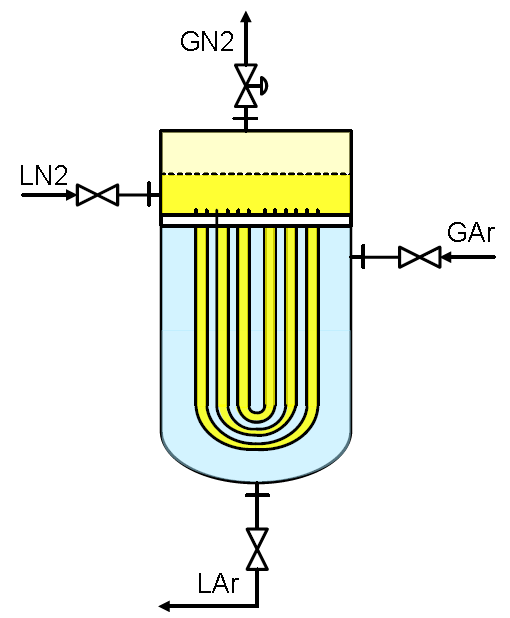
\includegraphics[width=.43\textwidth]{v5ch2-recondenser-2015}
\caption{Liquid argon recondenser}
\label{fig:v5ch2-recondenser-sept-2011}
\end{figure}

Each cryostat has a dedicated nitrogen-refrigeration plant 
and all four will be used for the initial cooldown and filling of the 
cryostats if possible because of the large volume of 
gas which must be cooled from 300 K to liquid
argon temperature (88.3$\pm$1 K). Further, each cryostat will
have four 85 kW condensers to 
provide the cooling power needed during initial 
cooldown and filling operations where warm GAr
is cooled and reliquefied to fill the cryostat.
After filling, only one condenser is needed with the
other providing redundancy.
This will ensure the high availability of the recondensing 
system and minimize the need for venting high-purity argon 
or allowing down-time for maintenance of
the recondensers and the refrigeration plants. 

\section{Argon Purification}
\label{subsec:argon-pur}
The cryostat is to be designed with side penetrations below the liquid level 
for external recirculation pumps used to continuously filter the cryostat's 
LAr. Figure~\ref{fig:external-pump} illustrates this mechanism. An Ebara 
model of vertical pump inserted into a vacuum insulated pump well, and 
external to the cryostat, is given 
as a typical example in Figure~\ref{fig:vert-submers-pumps}. The pump suction 
must be located at a small distance below the lowest liquid level 
(normally about 1.5 to 2~m above the bottom surface of the cryostat) 
to prevent cavitation and vapour-entrapment. The pumps and 
pump wells will extend as close to the bottom of the cryostat. They 
could also be staggered at different elevations to allow flexibility 
in drawing liquid from different 
elevations. Vertical cryogenic pumps are supplied by manufacturers 
such as Ebara and Carter Cryogenic Products. 

\begin{figure}[htbp]
\centering
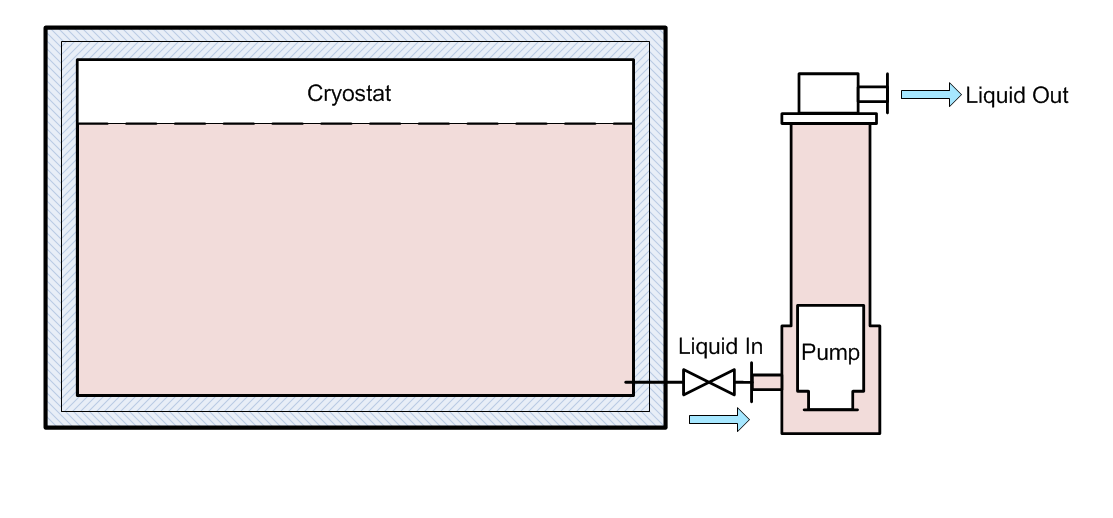
\includegraphics[width=.9\textwidth]{ExternalPumpSketch}
\caption{LAr recirculation mechanism using external pumps}
\label{fig:external-pump}
\end{figure}

\begin{figure}[htbp]
\centering
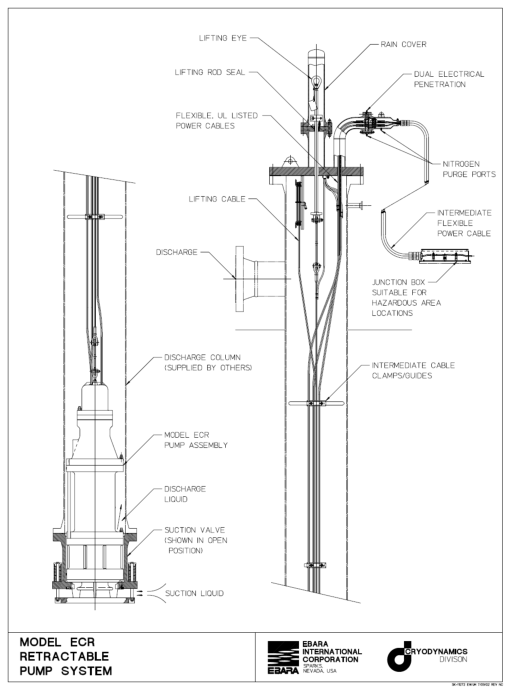
\includegraphics[width=.9\textwidth]{v5ch2-vert-submers-pumps}
\caption{Concept of vertical pump and well}
\label{fig:vert-submers-pumps}
\end{figure}

The required flow rate of liquid argon to be sent for purification 
is expected to decrease over time. The initial maximum flow rate 
will be 93~m$^3$/hr (411~gpm). The liquid-argon volume in one 
cryostat will turn over every 5.5 days at this rate. 
Longer term, the rate will decrease to 46~m$^3$/hr 
with a turn-over rate of 11 days.  As a point of comparison, ICARUS 
T600 has a maximum turn-over rate of about ten days. See the 
Table~\ref{table:purif-compare} for a comparison of purification 
rates among other experiments and LBNF. 
%To achieve the turn-down required between the short- and long-term flow rates, 
%two removable \textcolor{red}{25~m$^3$/hr (50?) (112~gpm) (224?)} pumps 
%will be located at the end of the cryostat. Placing the pumps at this 
%end of the cryostat will keep space clear for TPC installation. 
The purification skids are located in the central utility cavern.  
The multiple-pump arrangement will provide a very 
high level of redundancy, which will extend the maintenance-free 
operating period of the cryostat.  


The purification system consists of two types of filter vessels containing
 molecular-sieve and copper media filters. The filter is 1.0~m in 
diameter by 4.3~m tall. The filters are sized to provide effective 
media usage at low pressure drop (2~kPa or 0.3~psi) over the 
expected range of flow rates. One filter is for gas filtration 
during filling; the other type is for liquid filtration. After filling 
is complete, the gas filter can be repurposed for cryostat 
liquid filtration.

%The purifiers will be located \textcolor{red}{close to the cryostat} 
%to minimize both the volume of LAr in the circulation pipework 
%and the pump power required to achieve the desired flow rate.  
The cryostat liquid argon inventory is circulated through a purification 
filter to achieve and maintain the required purity. The purification filter,
 containing molecular sieve media to remove water and copper media to 
remove oxygen, will become saturated. The nearly saturated purification 
filter is regenerated to vent the contaminants. The liquid argon flow 
is switched to another purification filter for uninterrupted filtration. 

A purity monitor after the purification filter will monitor the filter 
effectiveness. (Purity monitors measuring electron lifetime will also 
be in the LAr bath and resident in the cryostat. It is a requirement 
that purity levels reach < 100 ppt oxygen equivalent to match the 
required electron lifetime of the detector). 

The regeneration of a filter is done in several steps. A saturated 
purification filter is first warmed with heated argon gas to an 
elevated temperature driving the captured water into the gas. 
Hydrogen gas is generated and mixed with the circulating argon 
gas up to 1.5\% hydrogen by volume. The hydrogen reacts with the 
oxygen and makes water that is also released into the circulating 
argon gas. Argon gas is vented to purge water from the hot 
circulating gas. 

The hot filter full of regenerated media is cooled by circulating 
chilled argon gas. The circulating argon gas is chilled first with 
a heat exchanger using a commercial R-404A refrigeration unit until 
the filter is cold. The commercial refrigeration unit accumulates 
the R-404A liquid and shuts down. The filter is next cooled down to 
cryogenic temperatures by circulating argon gas chilled by a second 
heat exchanger with a liquid nitrogen coolant. This completes the 
regeneration steps for a purification filter. The filter is now 
ready to be switched into service or held cold until needed. Two 
spare purification filters are used with separate heating and 
cooling loops to reduce the usage rate of electricity and liquid 
nitrogen. This also reduces the stresses on heat exchangers by 
decreasing their temperature swings.

\begin{table}
\caption{Purification comparision data for LArTPCs}
\label{table:purif-compare}
\centering
\rotatebox{90}{
\begin{tabular}[htbp]{|l|p{2.3cm}|p{2.3cm}|p{2.3cm}|p{2.3cm}|p{2.7cm}|}
\hline
\textbf{Experiment}  & \textbf{LAr Volume} & \textbf{Max Liquid}   & \textbf{Boil-off Gas} & \textbf{LAr Volume} & \textbf{Electron} \\
                     &                     & \textbf{Purification} & \textbf{Purification} & \textbf{Change}     & \textbf{Lifetime} \\
                     &                     & \textbf{Rate}         & \textbf{Rate}         & \textbf{Rate}       &                   \\
                     & \textbf{(m$^{3}$)}  & \textbf{(kg/hr)}      & \textbf{(kg/hr)}      & \textbf{(days)}     & \textbf{(milli-second)}  \\
\hline\hline
ICARUS T600          &  550 & 2766 &  168 & 10.8 &    > 5 \\
Detector             &      &      &      &      &      \\ 
\hline
ICARUS               &   10 &  692 & 0.69 &  0.8 &  1.1 \\
Prototype            &      &      &      &      &      \\
\hline
Material Test Stand  & 0.25 &  167 & 5.56 &  0.1 &  > 5 \\
      at FNAL        &      &      &      &      &      \\
\hline
ArgoNeut             & 0.55 &    0 & 4.3  &  7.3 & 0.75 \\
                     &      &      &      &      &      \\
\hline
Microboone           &  123 & 6875 &   83 &  0.9 & TBD  \\
                     &      &      &      &      &      \\
\hline
LAr Purity Demonstrator & 22.2 & 3791 & 46.7 &  0.3 & > 5  \\
(LAPD)               &      &      &      &      &      \\
\hline
LBNE 35 ton Membrane & 27.7 & 1900 &   27 &  0.7 & > 2.5 \\
Cryostat Prototype   &      &      &      &      &      \\
\hline
LBNF                 & 12452 & 129828 & 1328.26 &  5.5 & > 3.0 required \\
(Per Cryostat)       &      &      &      &      &      \\
\hline
\end{tabular} 
}
\end{table}

%\begin{figure}[htbp]
%\centering
%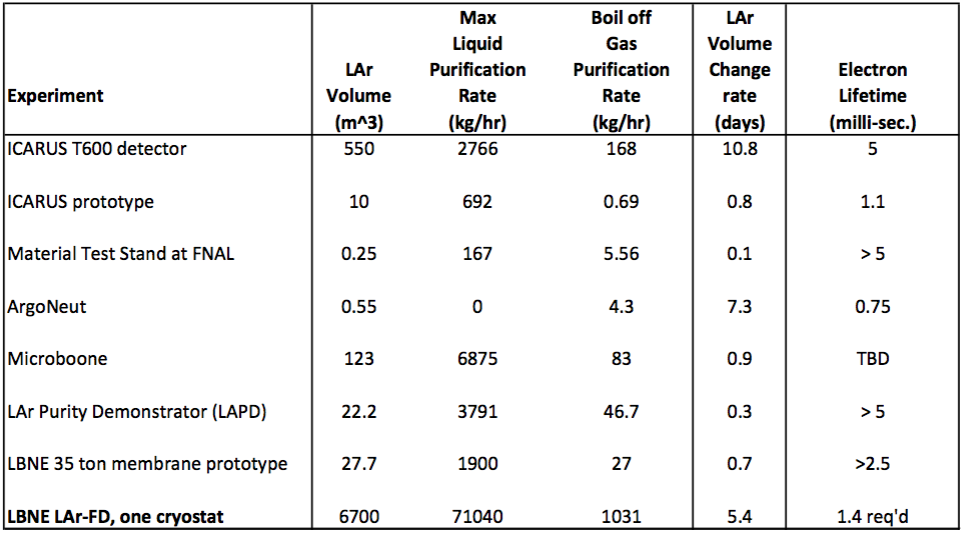
\includegraphics[width=.9\textwidth]{purification-comp-data-dec2014.png}
%\caption{Purification comparision data for LArTPCs}
%\label{fig:table:purif-compare}
%\end{figure}

\section{Pressure Control}
\label{sec:press-control}

\subsection{Normal Operations}

The pressure-control valves are sized and set to control the 
internal cryostat pressure under normal operating conditions 
to the nominal design pressure of 0.113~MPa. Fluctuations 
between 0.105~MPa (50~mbarg) and 0.121~MPa (200~mbarg) are 
intended to be the normal operating range.
%\fixme{note to self: put this unit in list of abbrevs}).  
Ten percent excursions above or below these levels will set off 
alarms to alert the operator to intervene. Further excursion 
may result in automatic (executive) actions.  These actions may 
include stopping the LAr circulation pumps (to reduce the heat 
ingress to the cryostat), increasing the argon flow rate through 
the recondenser, increasing the LN$_2$ flow through the recondenser vessel, 
powering down heat sources within the cryostat (e.g., detector electronics).  
Eventually, if the pressure continues to rise, it will trigger the 
pressure-relief valves to operate. Table~\ref{table:pressure-values} 
gives important pressure values.

%%%%%%%%%
\begin{table}
\centering
%\begin{tabular}[htbp]{| p{0.3\textwidth}|p{0.3\textwidth}||p{0.3\textwidth}|}
\caption{Important Pressure Values}
\label{table:pressure-values}\begin{tabular}[htbp]{|l|l|}
\hline 
Vessel ullage maximum operating pressure & 0.121 MPa, 200 mbarg, 2.9 psig\\
\hline
Cryostat Design Pressure; Relief valve set pressure& 0.135 MPa, 350 mbarg, 5.1 psig\\
\hline
\end{tabular} 

\end{table}
%%%%%%%%%

The ability of the control system to maintain a set pressure is 
dependent on the size of pressure deviations (due to changes in flow, 
heat load, temperature, atmospheric pressure, etc.) and the volume 
of gas in the system.  The reference design has 0.66 m 
of gas at the top of the cryostat.  This is 5\% of the total 
argon volume and is the typical vapor fraction used for cryogenic 
storage vessels. Reaction time to changes in the heat load is slow, 
on the order of an hour.  At the expected heat-load rate of 
69.9~kW, and for an isolated or un-cooled cryostat,
the rate of pressure rise would be 393~mbar (5.7 psi) per hour. 
Two redundant pressure control valves will
maintain the required pressure range, each sized to handle 
at least 1300 kg/hr of argon flow to the recondenser to handle 
the cooling and reliquefaction of warm GAr during cryostat filling.


\subsection{Overpressure Control}

In addition to the normal-operation pressure-control system, 
it is planned to provide a cryostat overpressure-protection 
system. This must be a high-integrity, automatic, failsafe
system capable of preventing catastrophic structural failure
of the cryostat in the case of excessive internal pressure.

The key active components of the planned system are pressure-relief 
valves (PRVs) located on the roof of the cryostat that will open rapidly when the differential pressure exceeds a 
preset value. A pressure-sensing line is used to trigger a pilot 
valve which in turn opens the PRV. A pressurized reservoir of 
power fluid is provided to each valve to ensure that the valves 
will operate under all deviation and/or shutdown scenarios. The PRVs 
are self-contained devices provided specially for cryostat protection; 
they are not normally part of the control system. 

The installation of the PRVs will ensure that each valve can 
periodically be isolated and tested for correct operation.  
The valves must be removable from service for maintenance 
or replacement without impacting the overall containment envelope 
of the cryostat or the integrity of the over-pressure protection 
system.  This normally requires the inclusion of isolation valves 
upstream and downstream of the pressure-relief valves and at least
one spare installed relief valve ($n+1$ provision).

When the valves open, argon is released, the pressure within the 
cryostat falls and argon gas discharges into the argon vent riser.  
The valves are designed to close when the pressure returns below 
the preset level.

\subsection{Vacuum-Relief System}

The cryostat vacuum-relief system is a high-integrity, 
automatic, failsafe system designed to prevent catastrophic 
structural failure of the cryostat due to low internal pressure.  
The vacuum-relief system protects the primary membrane tank. 
Activation of this system is a non-routine operation and is 
not anticipated to occur during the life of the cryostat. 

%Theoretically, 
Potential causes of reduced pressure in the cryostat include 
operation of discharge pumps while the liquid-return inlet 
valves are shut, gaseous argon condensing in the recondenser 
(a thermo-siphon effect), or a failure of the vent system 
when draining the cryostat. Vacuum-relief valves are provided 
on LNG/LPG storage tanks to protect the structure from these 
types of events.  


%A vacuum relief system will be provided in addition to the normal pressure-control system.   
The key active components of this additional protection system 
are vacuum-relief valves located on the roof of the cryostat 
that will monitor the differential pressure between the inside 
and the outside of the cryostat and open when the differential 
pressure exceeds a preset value, allowing cavern air to enter 
the cryostat to restore a safe pressure. 

\section{LN$_2$ Refrigeration System}
\label{sec:ln-refrig-sys}
%BN modified refrigeration size 10/6/2011
Four commercial LN$_2$-refrigeration plants will be procured for LBNF.  
After achieving the required purity and completing the initial fill, each 
cryostat will have a dedicated LN$_2$ plant for steady-state operations.
The plants will be located in the central utility cavern at the 
4850L. Each will be a closed-loop system supplying LN$_2$
to the argon recondenser. The nominal rating of the quoted
refrigerators is in the range of 71 kW.

Two-phase nitrogen is delivered from the cold end of the refrigerator 
into a farm of  LN$_2$ storage vessels with a total capacity of 50 m$^3$ per cryostat. 
Pure liquid is withdrawn from the LN$_2$ storage vessels and is supplied 
via a transfer line to a pressure-reducing valve and phase-separator tank 
also located within the central utility cavern. LN$_2$ is then withdrawn from the bottom 
of the phase-separator tank, at a pressure of 2.0 bar and temperature of 
84 K, and directed to the recondenser. This results in a 5 K temperature 
difference relative to the 89 K argon recondenser temperature. The 
six 8.3 m$^3$ LN$_2$ vessels will allow for greater than forty hours 
of refrigeration time. This time window is adequate to cover most power 
outages, refrigerator performance problems and refrigerator switch-overs.

The refrigeration system operation, illustrated in Figure~\ref{fig:LN2-refrigerator-flow}, 
is based on a screw compressor package and three turbo expanders. 
This system is expected to be capable of running  
continuously for at least a year, and then require only 
minor servicing. The system will be equipped with 
automatic controls and a remote monitoring so that no operator 
will be required during normal operation. 
Estimated maximum power requirement is 1500 hp (1119 kVA), 
not taking into account the power generated by the expanders.  
The LBNF reference design places the nitrogen compressor in 
a surface-level equipment building. A closed-loop water system 
with evaporative-cooling tower removes heat from the compressor. 
Compression is carried out at close-to-ambient temperature. 
A compressor aftercooler is provided to reject heat. 

\begin{figure}[htbp]
\centering
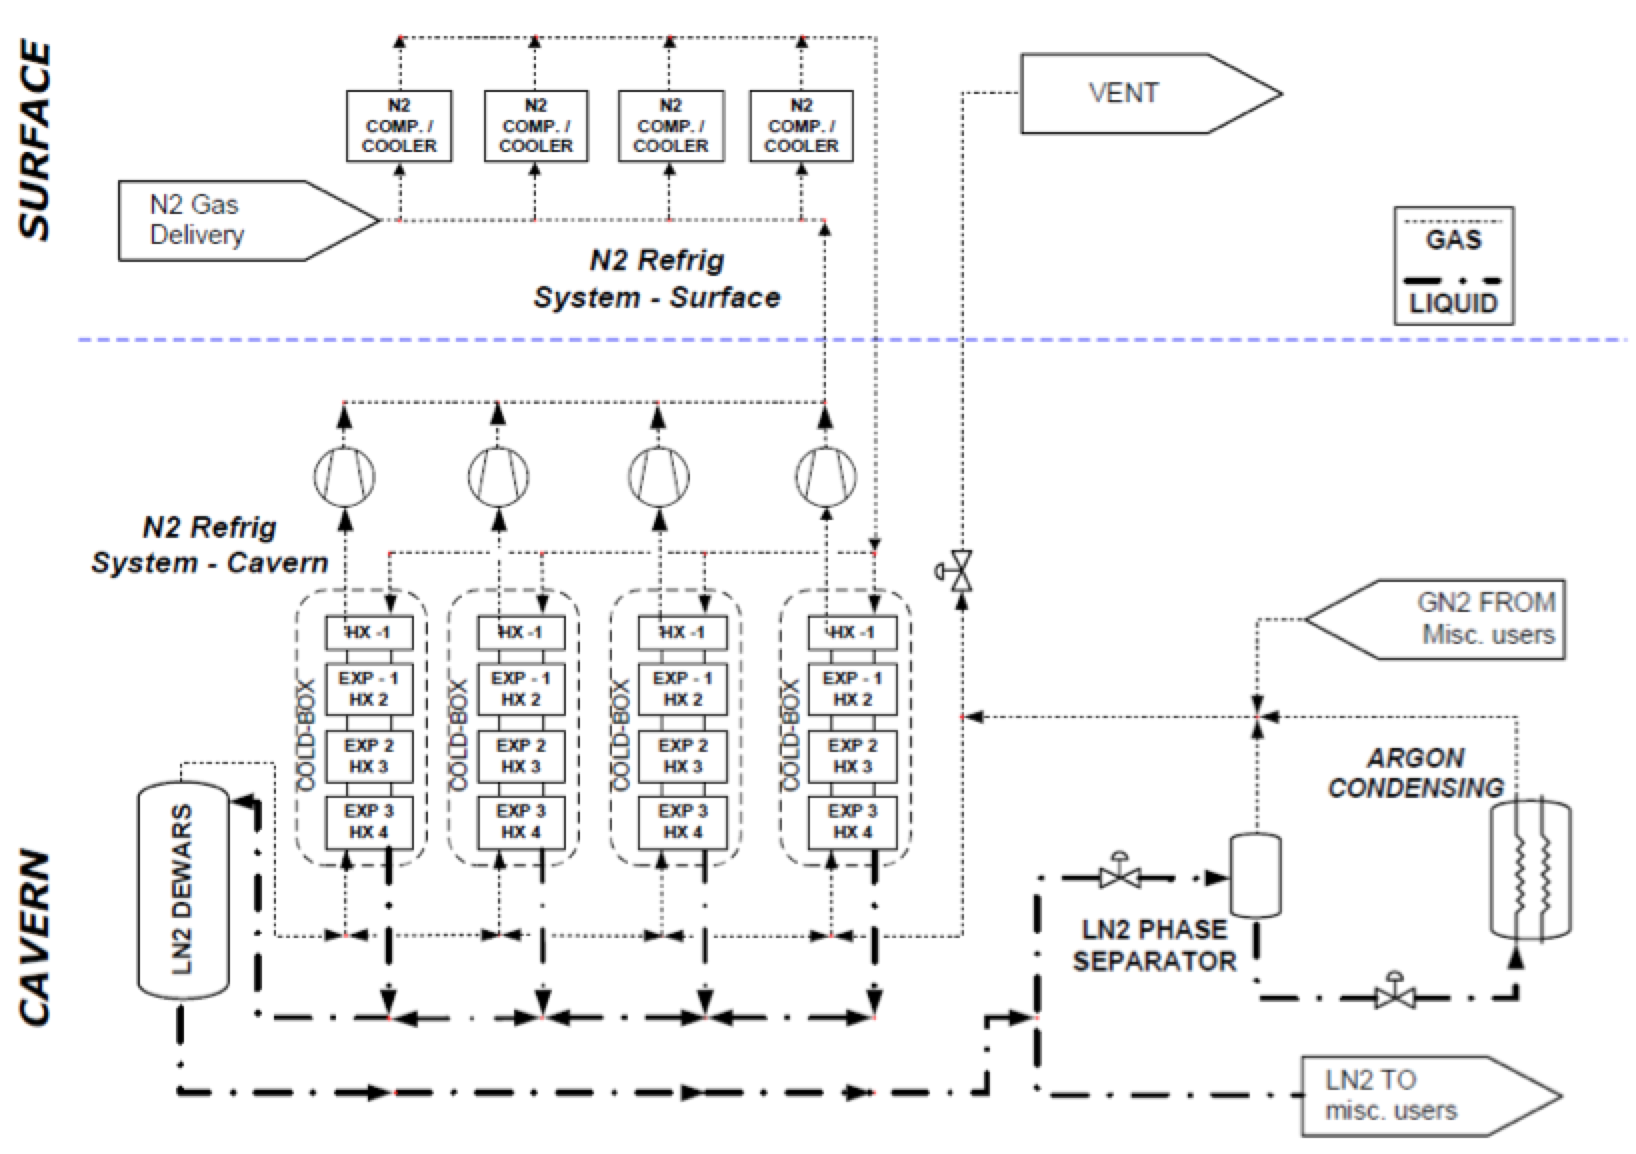
\includegraphics[width=1.25\textwidth,angle=270]{nitrogen-refrig-plant-flow.png}
\caption{Nitrogen refrigeration-plant flow diagram}
\label{fig:LN2-refrigerator-flow}
\end{figure}

The fluid is next routed to a `cold box' consisting of four heat exchangers.  
This series of exchangers provides staged heat transfer from a cooling 
nitrogen stream to a warming one.  The expanders are connected between 
the heat exchangers to progressively reduce the pressure of the cooling 
nitrogen stream to isentropically reduce the pressure and temperature of the
nitrogen stream, eventually leading to a large liquid-nitrogen fraction 
at the coldest end of the cold box. 

The main cold box shell is 1.22~m (4~ft) in diameter and 8.2~m (27~ft) tall, 
as illustrated in Figure~\ref{fig:nitrogren-refrigerator}. The expanders 
are adjacent to the cold box at three elevations and extend about 1~m to
the side of the cold box shell. The reference design cold box weighs 5670~kg. The 
compressors are located at the surface inside an equipment building. 
The compressor skid (frame) is 4.3~m long, 1.8~m wide and 2.7~m tall 
and weighs approximately 3630~kg.  

\begin{figure}[htbp]
\centering
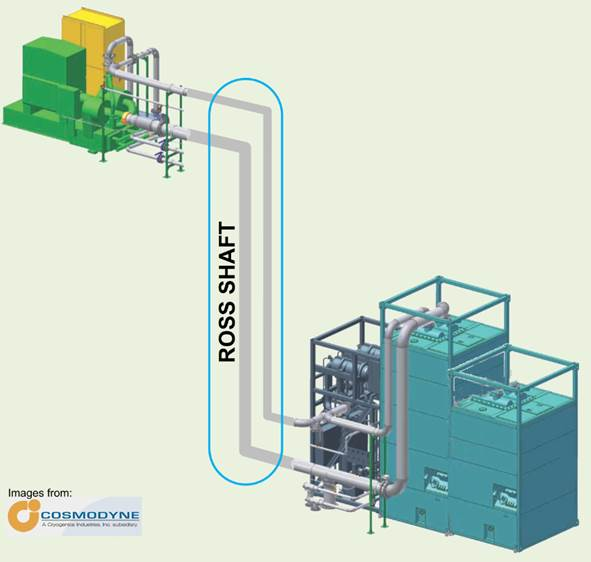
\includegraphics[width=.7\textwidth]{refrigplant}
\caption{Nitrogen refrigeration plant (not to scale)}
\label{fig:nitrogren-refrigerator}
\end{figure}

\section{Refrigeration Load Scenarios}
\label{sec:refrigeration-load-scenarios}

%\begin{editornote}
%Editor's Note:  The load scenario information contained in this section 
%is relevant for a 34-kton fiducial mass detector made up of two 17-kton 
%modules.  As of late 2014, the refrigerator will need to serve the first 
%10-kton detector cavern and the 30-kt detector cavern.
%\end{editornote}

In order to determine the optimal plant capacity and number of plants 
required, fourteen scenarios were forecasted for the LN$_2$ refrigeration
loads and plant capacity.  Those scenarios are described below and 
a summary is given in Table~\ref{table:Refrigeration-loads}. 
                          
The conclusion points to the requirement of four 71 kW plants. Each of 
these plants can achieve a 20\% turn up or turn down. Scenarios 1, 4, 
A and D impose the most severe requirements. In these scenarios, all 
plants available will be required to run at the maximum duty cycle 
to cool down and fill a cryostat, while maintaining purity for
cryostat(s) filled and purified earlier. These scenarios will
also require frequent filter regeneration.

\begin{description}
\item[Scenario 1]
The initial operation will be the purging, cooling and filling of the 
first cryostat, condensing gaseous argon in the cavern by heat exchange 
via the recondensers. The surface and cavern LAr and  LN$_2$ dewars 
will be operational and the cooling load for the dewars will come 
directly from the refrigeration plant. The cavern pipework and vessels 
will be cold, the LAr in the cryostat will be circulating at high flow 
rate through the purification plant, and the cryostat will be cold.
The cryostat cool-down rate is constrained by three variables: 1) The 
size of the piping from the surface to bottom of Ross shaft, 2) The 
size of the LN$_2$ refrigeration units, and 3) the cooling power 
available via the recondensers.  All three variables have been 
matched for the physical constraints of a 40 kton module at 4850L 
using the Ross shaft. The refrigerators and condensers have been 
sized to accommodate the long-term refrigeration load associated 
with the cryostats.  As the LAr is circulated to achieve the 
operational purity the filtration plant will need to be regularly 
regenerated. This will mean that the associated refrigeration 
load will normally be present.

\item[Scenario 2]
Once the first cryostat is filled with LAr, the cool-down load will 
reduce to zero and the cryogenic plant will run for several months 
purifying the LAr inventory.

\item[Scenario 3]
When the LAr in the cryostat reaches the required purity level, the 
circulation flow rate will be reduced and the detector electronics 
will be turned on.  At this stage the recondenser refrigeration 
load falls such that only one recondenser is required and the 
rest of units can operate as spare units.

\item[Scenario 4] The first cryostat continues to operate in normal
experimental mode 
%and 
while  the second cryostat is being purged, cooled down and 
filled with LAr. Again a very large burden is placed on the 
recondensers due to the gas condensation and rate of liquefaction.

\item[Scenario 5] The second cryostat is full and LAr is circulated 
at high flow rate through the purification plant. The first cryostat
continues to operate as normally.

\item[Scenario 6]
Both cryostats are operating in normal experimental mode. A spare 
recondenser is available on each cryostat to facilitate maintenance.

\item[Scenario 7]
It is assumed that a total failure of the refrigeration plant has 
occurred. All noncritical heat sources are isolated and liquid 
nitrogen from the LN$_2$ vessels in the central utility cavern 
is utilized to recondense the inventory of high purity LAr. Nitrogen 
refrigeration must be reestablished before the liquid nitrogen reservoir 
is exhausted or the high purity argon will need to be vented. In the 
locked-down state, the recirculation pumps and the purification 
plants are shut down.

\item[Scenario A]
The first and second cryostats continue to operate in normal
experimental mode while  the third cryostat is being purged, 
cooled down and filled with LAr. Again a very large burden 
is placed on the recondensers due to the gas condensation 
and rate of liquefaction.

\item[Scenario B]
The third cryostat is full and LAr is circulated at high 
flow rate through the purification plant. The first and 
second cryostats continue to operate as normally.

\item[Scenario C]
Three cryostats are operating in normal experimental mode. A spare 
recondenser is available on each cryostat to facilitate maintenance.

\item[Scenario D]
The three cryostats continue to operate in normal experimental
mode while the fourth cryostat is being purged, cooled down 
and filled with LAr. Again a very large burden is placed 
on the recondensers due to the gas condensation 
and rate of liquefaction.

\item[Scenario E]
The fourth cryostat is full and LAr is circulated at high 
flow rate through the purification plant. The three cryostats 
previously filled continue to operate as normally.

\item[Scenario F]
All four cryostats are operating in normal experimental mode. A spare 
recondenser is available on each cryostat to facilitate maintenance.

\item[Scenario G]
This is the same condition as Scenario 7, but now all four cryostats
are in the LAr inventory protection mode.

\end{description}
 
\begin{table}
\centering
\rotatebox{90}{
\scriptsize
%\tiny
\begin{tabular}[htbp]{|l|c|c|c|c|c|c|c|c||c|c|c|c|c|c|c|}
\hline
                     & \textbf{Unit}  & \multicolumn{14}{c|}{\textbf{Scenarios}} \\
\cline{3-16}
\textbf{Heat Demand} & \textbf{Loads} &   &   &   &   &   &   &   &   &   &   &   &   &   &   \\
                     & \textbf{(kW)}  & 1 & 2 & 3 & 4 & 5 & 6 & 7 & A & B & C & D & E & F & G \\
\hline\hline
\multicolumn{16}{|c|}{\textbf{Recondenser Load, Cryostat \#1}}                          \\
\hline
Cryostat \#1, Heat Ingress & 32.1 & 32.1 & 32.1 & 32.1 & 32.1 & 32.1 & 32.1 & 32.1 & 32.1 & 32.1 & 32.1 & 32.1 & 32.1 & 32.1 & 32.1 \\     
With 2 Recirculation Pumps & 10.4 &      &      & 10.4 & 10.4 & 10.4 & 10.4 &      & 10.4 & 10.4 & 10.4 & 10.4 & 10.4 & 10.4 & \\ 
With 4 Recirculation Pumps & 20.7   & 20.7 & 20.7 &      &      &      &      &      & & & & & & & \\ 
Piping \& Purification Vessel Heat Ingress & 3.7 & 3.7 & 3.7 & 3.7 & 3.7 & 3.7 & 3.7 &   & 3.7 & 3.7 & 3.7 & 3.7 & 3.7 & 3.7 &      \\
Detector Electronics in Cryostat & 23.7 & & & 23.7 & 23.7 & 23.7 & 23.7 &   & 23.7 & 23.7 & 23.7 & 23.7 & 23.7& 23.7 &        \\
Cryostat Fill - GAr Transfer/Recondense &  & 190.48 & & & & & & & & & & & & &               \\
\hline
Number of Condensers in Operation & & 3 & 1 & 1 & 1 & 1 & 1 & 1 & 1 & 1 & 1 & 1 & 1 & 1 & 1\\
\textbf{Condenser Load} & & 247.0 & 56.5 & 69.9 & 69.9 & 69.9 & 69.9 & 32.1 & 69.9 & 69.9 & 69.9 & 69.9 & 69.9 & 69.9 & 32.1 \\
\hline\hline
\multicolumn{16}{|c|}{\textbf{Recondenser Load, Cryostat \#2}} \\
\hline
Cryostat \#2, Heat Ingress & 32.1 &    &   &   & 32.1 & 32.1 & 32.1 & 32.1 & 32.1 & 32.1 & 32.1 & 32.1 & 32.1 & 32.1 & 32.1 \\     
With 2 Recirculation Pumps & 10.4 &      &      &      &      &      & 10.4 &   & 10.4 & 10.4 & 10.4 & 10.4 & 10.4 & 10.4 &   \\ 
With 4 Recirculation Pumps & 20.7 &      &      &      & 20.7 & 20.7 &      &   & & & & & & &   \\ 
Piping \& Purification Vessel Heat Ingress & 3.7 &   &   &   & 3.7 & 3.7 & 3.7 &  & 3.7 & 3.7 & 3.7 & 3.7 & 3.7 & 3.7 &       \\
Detector Electronics in Cryostat & 23.7 &   &   &   &   &   & 23.7 &   & 23.7 & 23.7 & 23.7 & 23.7 & 23.7 & 23.7 &        \\
Cryostat Fill - GAr Transfer/Recondense & &  & & & 120.62 & & &  & & & & & & &              \\
\hline
Number of Condensers in Operation & &  &  &  & 3 & 1 & 1 & 1 & 1 & 1 & 1 & 1 & 1 & 1 & 1 \\
\textbf{Condenser Load} & &   &   &   & 177.1 & 56.5 & 69.9 & 32.1 & 69.9 & 69.9 & 69.9 & 69.9 & 69.9 & 69.9 & 32.1 \\
\hline\hline
\multicolumn{16}{|c|}{\textbf{Recondenser Load, Cryostat \#3}}                          \\
\hline
Cryostat \#3, Heat Ingress & 32.1 &  & &  &  &  &  &  & 32.1 & 32.1 & 32.1 & 32.1 & 32.1 & 32.1 & 32.1 \\     
With 2 Recirculation Pumps & 10.4  &   &   &  &   &   &   &   & & & 10.4 & 10.4 & 10.4 & 10.4 & \\ 
With 4 Recirculation Pumps & 20.7 &   &   &  &    &  &  &  & 20.7 & 20.7 & & & & & \\ 
Piping \& Purification Vessel Heat Ingress & 3.7 &  &  &  &  &  &  &  & 3.7 & 3.7 & 3.7 & 3.7 & 3.7 & 3.7 &       \\
Detector Electronics in Cryostat & 23.7  & & & & &  &  &  & & & 23.7 & 23.7 & 23.7 & 23.7 &         \\
Cryostat Fill - GAr Transfer/Recondense & & & & & & & & & 135.76 & & & & & &               \\
\hline
Number of Condensers in Operation & &  &  &  &  &  &  &  & 3  & 1 & 1 & 1 & 1 & 1 & 1 \\
\textbf{Condenser Load} & &   &   &   &   &   &   &   & 192.3 & 56.5 & 69.9 & 69.9 & 69.9 & 69.9 & 32.1 \\
\hline\hline
\multicolumn{16}{|c|}{\textbf{Recondenser Load, Cryostat \#4}} \\
\hline
Cryostat \#4, Heat Ingress & 32.1 &  &   &   &  &  &  &  & & & & 32.1 & 32.1 & 32.1 & 32.1\\     
With 2 Recirculation Pumps &  10.4 &      &      &      &      &      &      &  & & & & & & 10.4 &    \\ 
With 4 Recirculation Pumps & 20.7 &      &      &      &      &      &      &  & & & & 20.7 & 20.7 & &    \\ 
Piping \& Purification Vessel Heat Ingress & 3.7 &   &   &   &  &  &  &   & & & & 3.7 & 3.7 & 3.7 &      \\
Detector Electronics in Cryostat & 23.7 &   &   &   &   &   &  &   & & & & & & 23.7 &        \\
Cryostat Fill - GAr Transfer/Recondense &   &  & & &  & & & & & & & 65.90 & & &               \\
\hline
Number of Condensers in Operation & &  &  &  &  &  &  &  & & & & 2 & 1 & 1 & 1 \\
\textbf{Condenser Load} & &   &   &   &   &   &   &  & & & & 122.4 & 56.5 & 69.9 & 32.1 \\
Cavern LN$_2$ Dewar Heat Ingress & 8 & 8 & 8 & 8 & 8 & 8 & 8 & & 8 & 8 & 8 & 8 & 8 & 8 & \\
\hline\hline
%LN$_{2}$ Storage Dewar Recondenser & 2 & 2 & 2 & 2 & 2 & 2 & 2 & & & & & & & & \\
Refrigeration Needed & & 255.0 & 64.5 & 77.9 & 255.0 & 134.4 & 147.7 & 64.2 & 340.0 & 204.2 & 217.6 & 340.0 & 274.1 & 287.4 & 128.4 \\
Refrigeration Plants in Operation & & 3 & 3 & 3 & 3 & 3 & 3 & 0 & 4 & 4 & 4 & 4 & 4 & 4 & 0 \\
Total Refrigeration Capacity Available & & 255 & 255 & 255 & 255 & 255 & 255 & & 340 & 340 & 340 & 340 & 340 & 340 & \\
Required Duty per Plant & & 85 & 60 & 60 & 85 & 60 & 60 & & 85 & 60 & 60 & 85 & 69 & 72 & \\
%Actual Duty per Plant & & & & & & & & & & & & & & & \\
Electric Trim Heater Load & & 0.0 & 115.5 & 102.1 & 0.0 & 45.6 & 32.3 & & 0.0 & 35.8 & 22.4 & 0.0 & 0.0 & 0.0 & \\
Total Refrigeration Load & & 255 & 180 & 180 & 255 & 180 & 180 & 0 & 340 & 240 & 240 & 340 & 274.1 & 287.4 & 0 \\
\hline\hline
LAr Mass in Cryostat & & 17129778 & & & 17129778 & & & & 17129778 & & & 17129778 & & & kg \\
Fill Time Using Available Cooling Above & & 4002 & & & 6321 & & & & 5616 & & & 11569 & & & hr \\
(Units Listed on the right-most column & & 167.0 & & & 263.0 & & & & 234.0 & & & 482.0 & & & days \\
of table) & & 23.8 & & & 37.6 & & & & 33.4 & & & 68.9 & & & weeks \\ 
& & 5.5 & & & 8.7 & & & & 7.7 & & & 15.9 & & & months \\
\hline  
\end{tabular} 
}
\caption{Refrigeration loads}
\label{table:Refrigeration-loads}
\end{table}


%\begin{figure}[htbp]
%\centering
%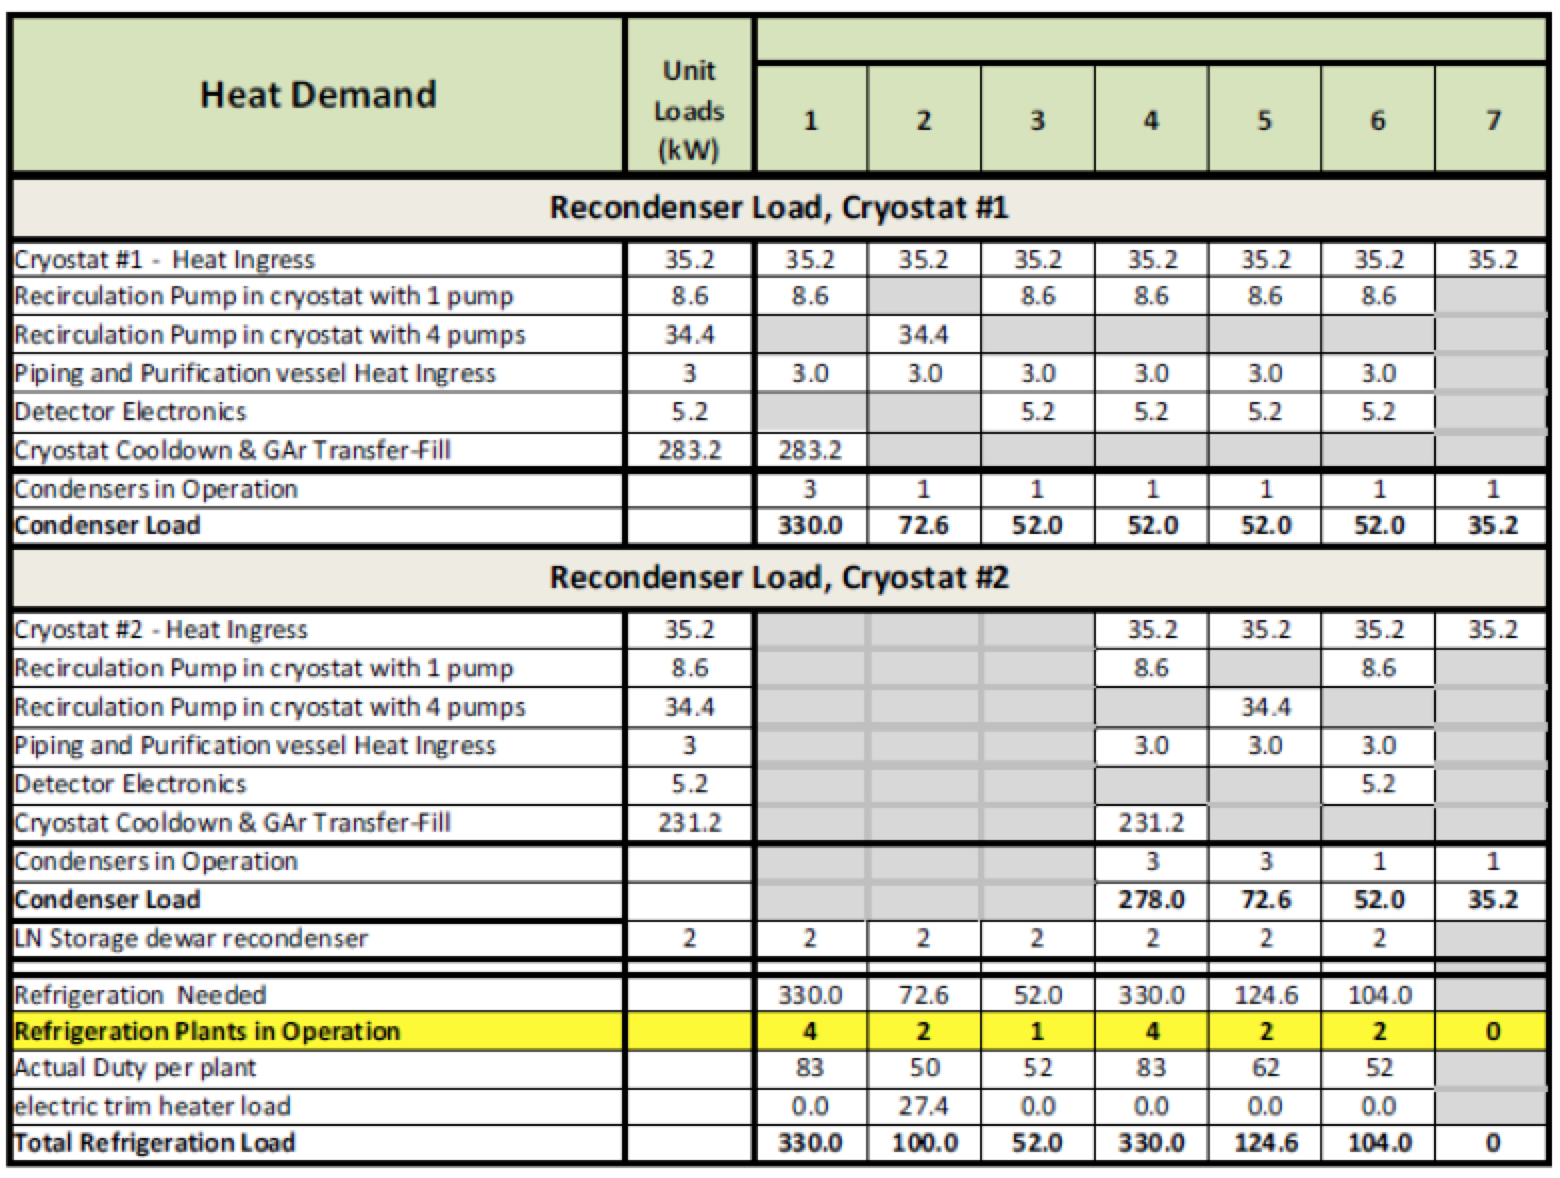
\includegraphics[width=\textwidth, angle = 90]{refrig-loads.png}
%\caption{Refrigeration loads}
%\label{fig:Refrigeration-loads}
%\end{figure}

%\begin{figure}[htbp]
%\centering
%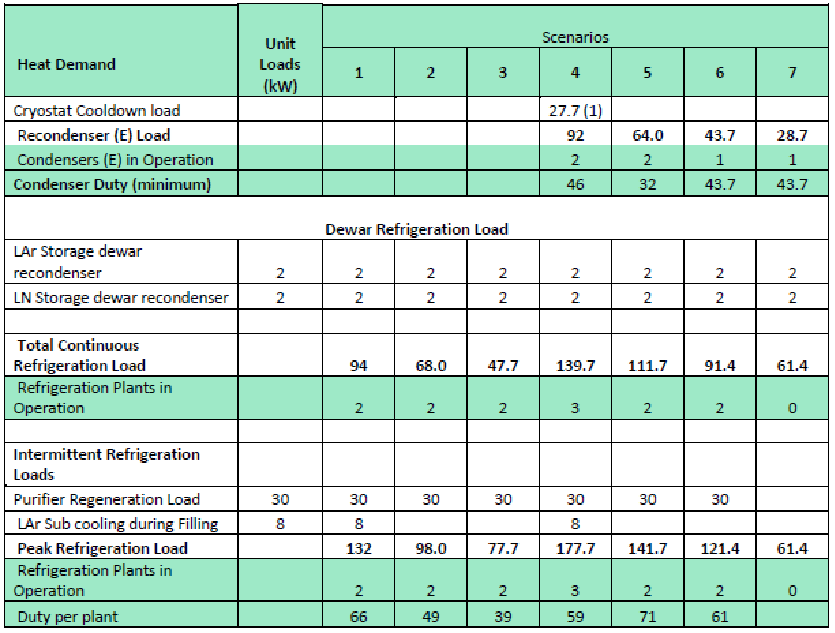
\includegraphics[scale=1, angle = 90]{v5ch2-arup-refrigeration-loads-fig2}
%\caption{Refrigeration loads, continued}
%\label{fig:Refrigeratior-loads-2}
%\end{figure}


\chapter{Prototyping Plans}
\label{sec:cryo-cryosys-proto-plans}

%\begin{editornote}
%Editor's Note: LAPD has successfully achieved greater than 5 millisecond 
%electron lifetime, and the LBNE 35 t has also achieved greater than 
%2.5 milli-second electron lifetime. 
%\end{editornote}

The development of the LBNF cryogenics infrastructure from conceptual 
to preliminary design includes a prototyping program. The most 
significant issue to resolve is whether a membrane cryostat in
the size of LBNF can achieve the required electron drift lifetime. 
The Liquid Argon Purity Demonstrator (LAPD) was an 
off-project prototype, built to study the concept of achieving
LAr purity requirements in a non-evacuated vessel. 
The purge process accomplished in the LAPD was 
repeated on the 35 ton membrane-cryostat prototype 
developed as an LBNE effort, which confirmed that initial 
evacuation of the cryostat is unnecessary and that 
a LAr purity level sufficient to enable the electron lifetime 
required in a membrane cryostat can be achieved~\cite{Montanari:2013/06/13aqa}.
Further prototyping program aiming to test and demonstrate 
this technology at the 1 kton scale is foreseen over the
next two years as part of the CERN Neutrino Platform program.

\chapter{ES\&H}
\label{sec:cryo-cryosys-esh}

Figure~\ref{fig:ODH-mapping-4850L} shows the ODH classification for
underground caverns. The detector and central utility caverns
are Class 1 ODH areas~\cite{feshm},
%based on fatality rate
%per hour (10$^{-7}$/hr < P(F) < 10$^{-5}$/hr)
assessed by preliminary ODH analysis taking into account
potential risks from undetected defects on materials
and equipment, operational causes, etc.
%with respect to the usage of argon, nitrogen
%and hydrogen.
During an ODH event, workers must leave the area heading towards the Ross or Yates shaft.

\begin{figure}[htbp]
\centering
\includegraphics[width=0.75\textwidth]{ODH-Mapping-4850L}
\caption{ODH mapping of the underground caverns at 4850L} 
\label{fig:ODH-mapping-4850L}
\end{figure}

During all phases of LBNF and the proposed prototypes, 
Fermilab ES\&H standards and Sanford Underground Research 
Facility (SURF) ES\&H codes and standards will guide the design, 
procurement and installation phases of the project. Particular 
attention will be paid to critical sections of
Chapter 4240~\cite{feshm} relating to ODH and 
Chapter 5000~\cite{feshm} standards for 
piping construction and vessel design. The planned 
work process will provide for reviews throughout all 
phases of the project to guarantee stringent adherence 
to the safety requirements. Requirements on the membrane-cryostat
materials and their fabrication will be strictly outlined in the 
specification documents. Close communication between the vendors, 
Fermilab and CERN's cryogenic and process engineers, and Fermilab and 
SURF ES\&H personnel will be maintained at all times.
